
\chapter{Sigma}
\newpage

\section{lecture}

\subsection{SIGMA}
Sigma is a generic and open signature format that allows you to describe relevant log events in a straightforward manner. The rule format is very flexible, easy to write and applicable to any type of log file. The main purpose of this project is to provide a structured form in which researchers or analysts can describe their once developed detection methods and make them shareable with others.

Sigma is for log files what Snort is for network traffic and YARA is for files.

\begin{center}
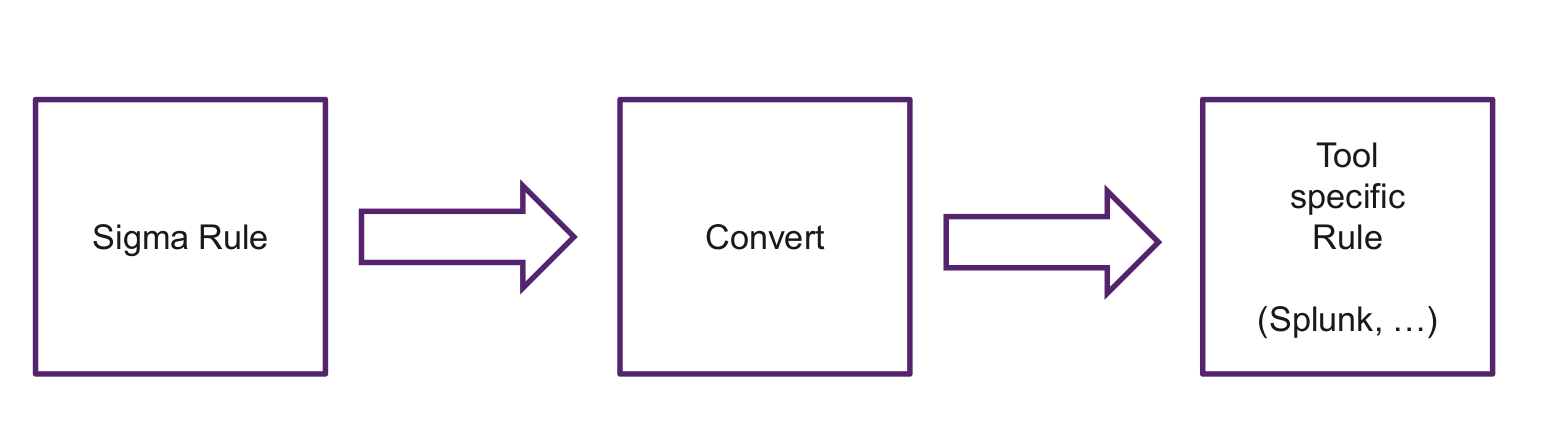
\includegraphics[width=\textwidth]{resources/12-sigma-01.png}
\end{center}

\subsubsection{Detection Rules: Sigma}
\begin{itemize}
  \item Widely accepted
  \item Platform agnostic (avoid vendor lock in)
  \begin{itemize}
    \item Has tooling to convert to your environment
    \item Great library of rules
    \item Community driven!
  \end{itemize}
\end{itemize}

\subsubsection*{Structure}
\begin{itemize}
  \item It is relatively simple to use
  \item Yet very powerful
  \item Let’s look at the specification and then some examples!
\end{itemize}
\begin{center}
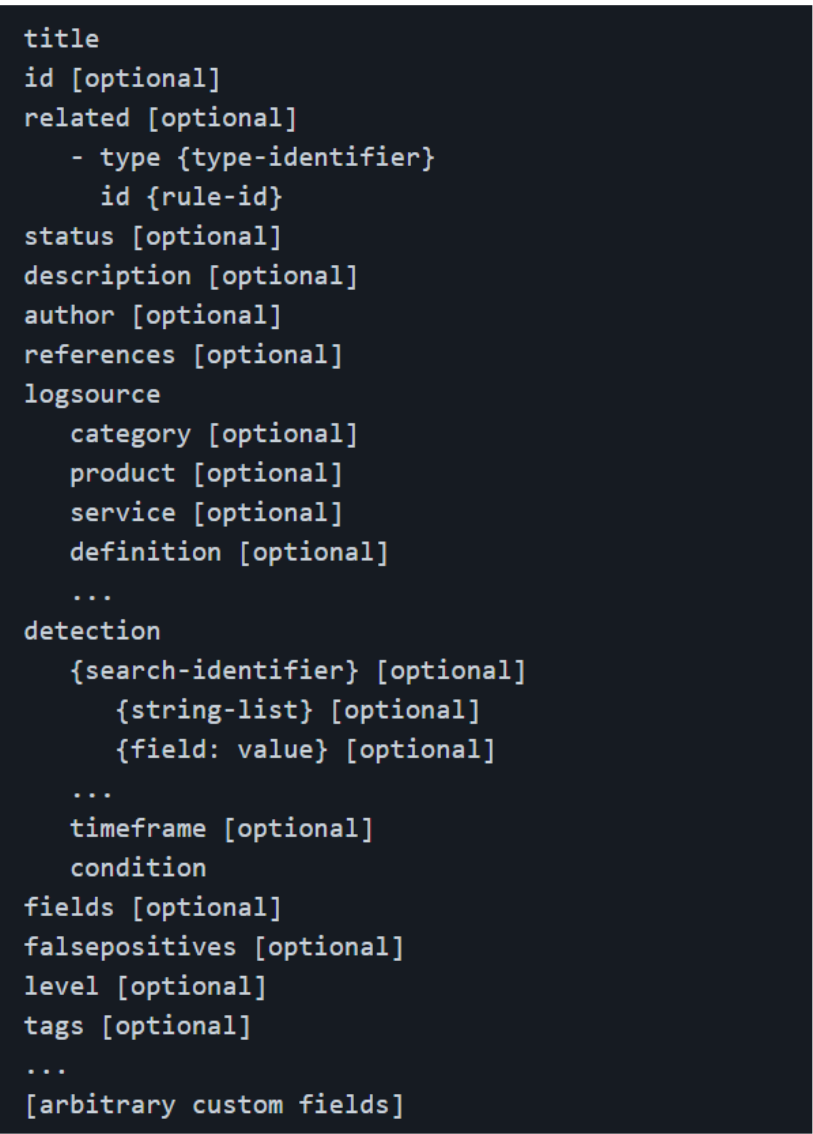
\includegraphics{resources/12-sigma-structure.png}
\end{center}

\begin{center}
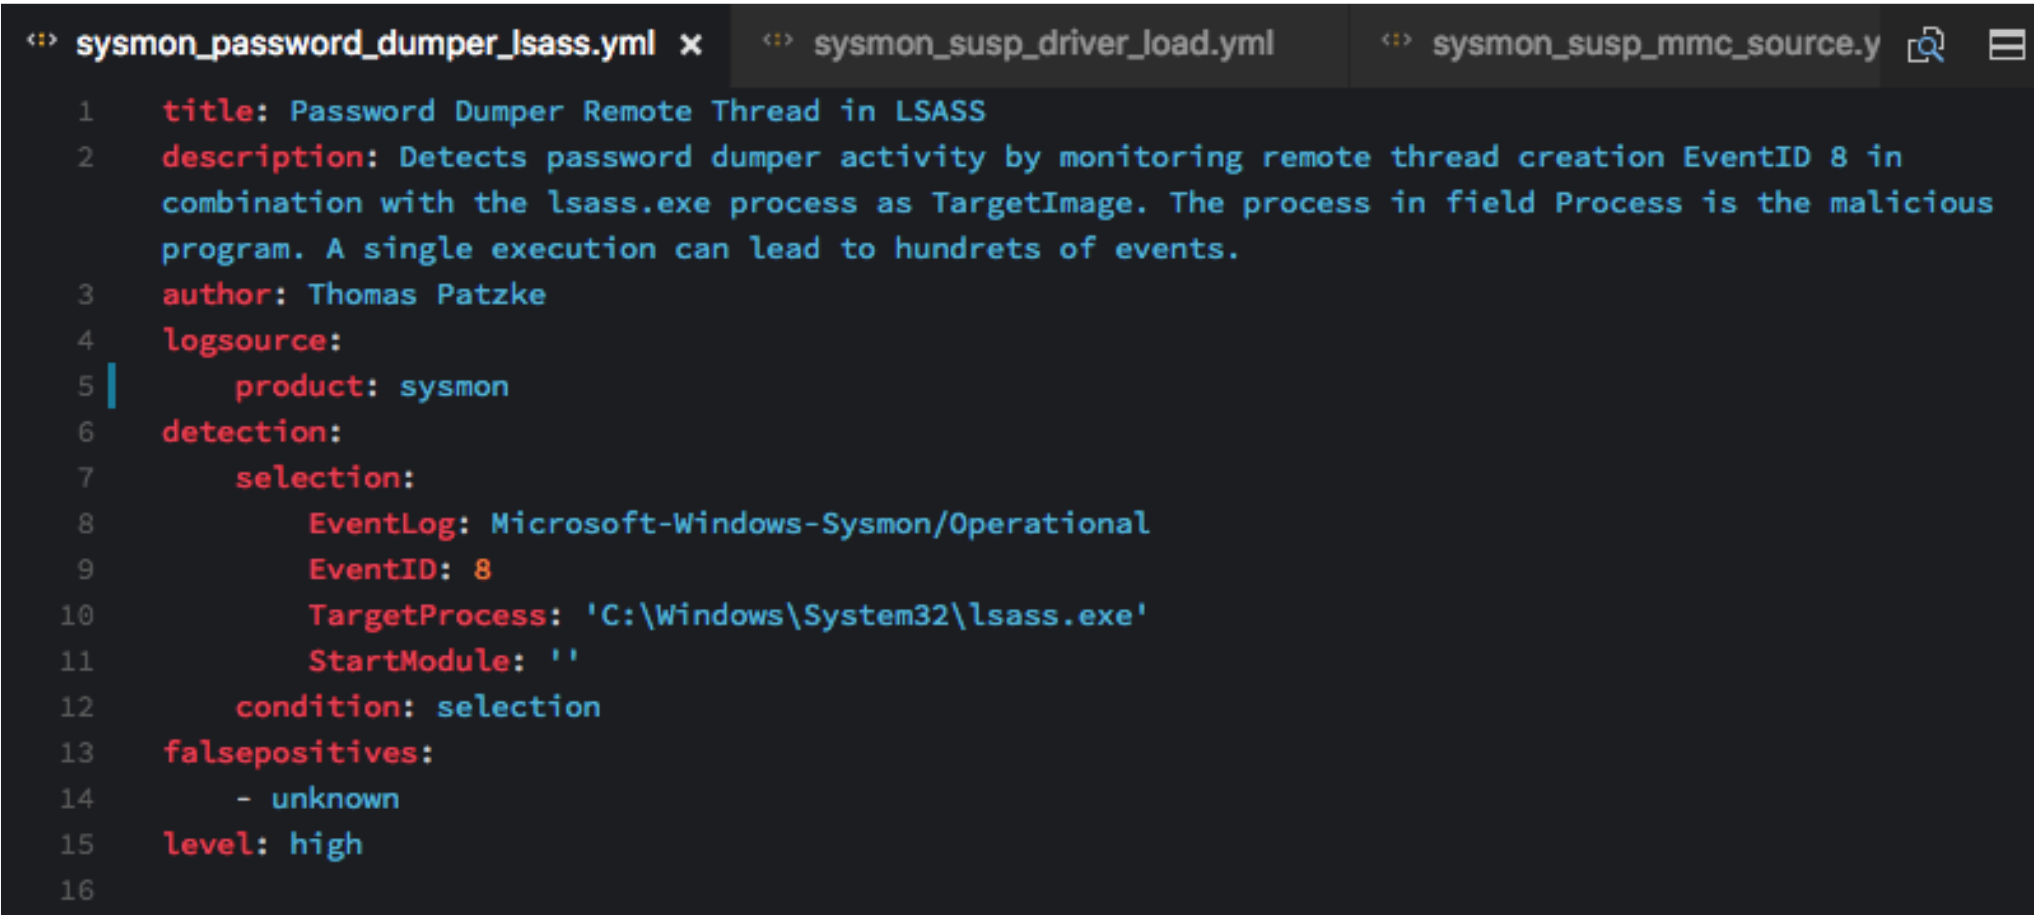
\includegraphics[width=\textwidth]{resources/12-sigma-detection-rules.png}
\end{center}

\begin{center}
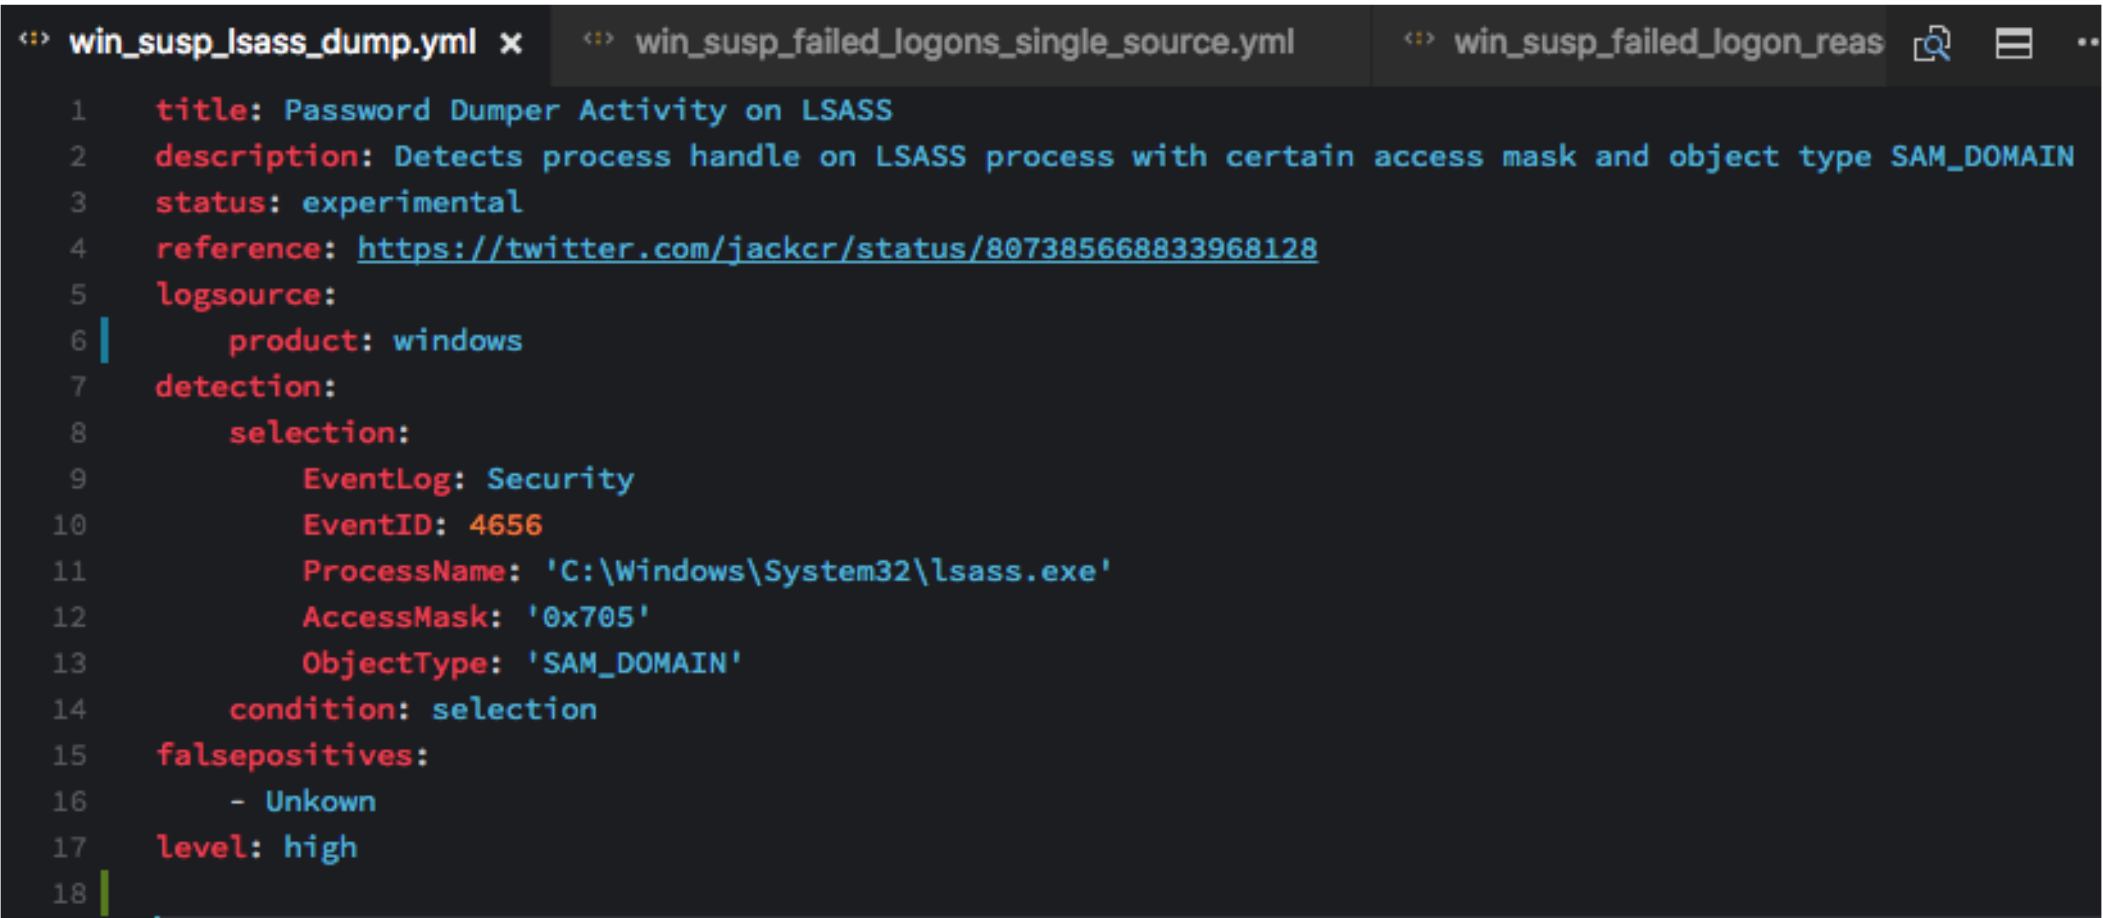
\includegraphics[width=\textwidth]{resources/12-sigma-detection-2.png}
\end{center}

\begin{center}
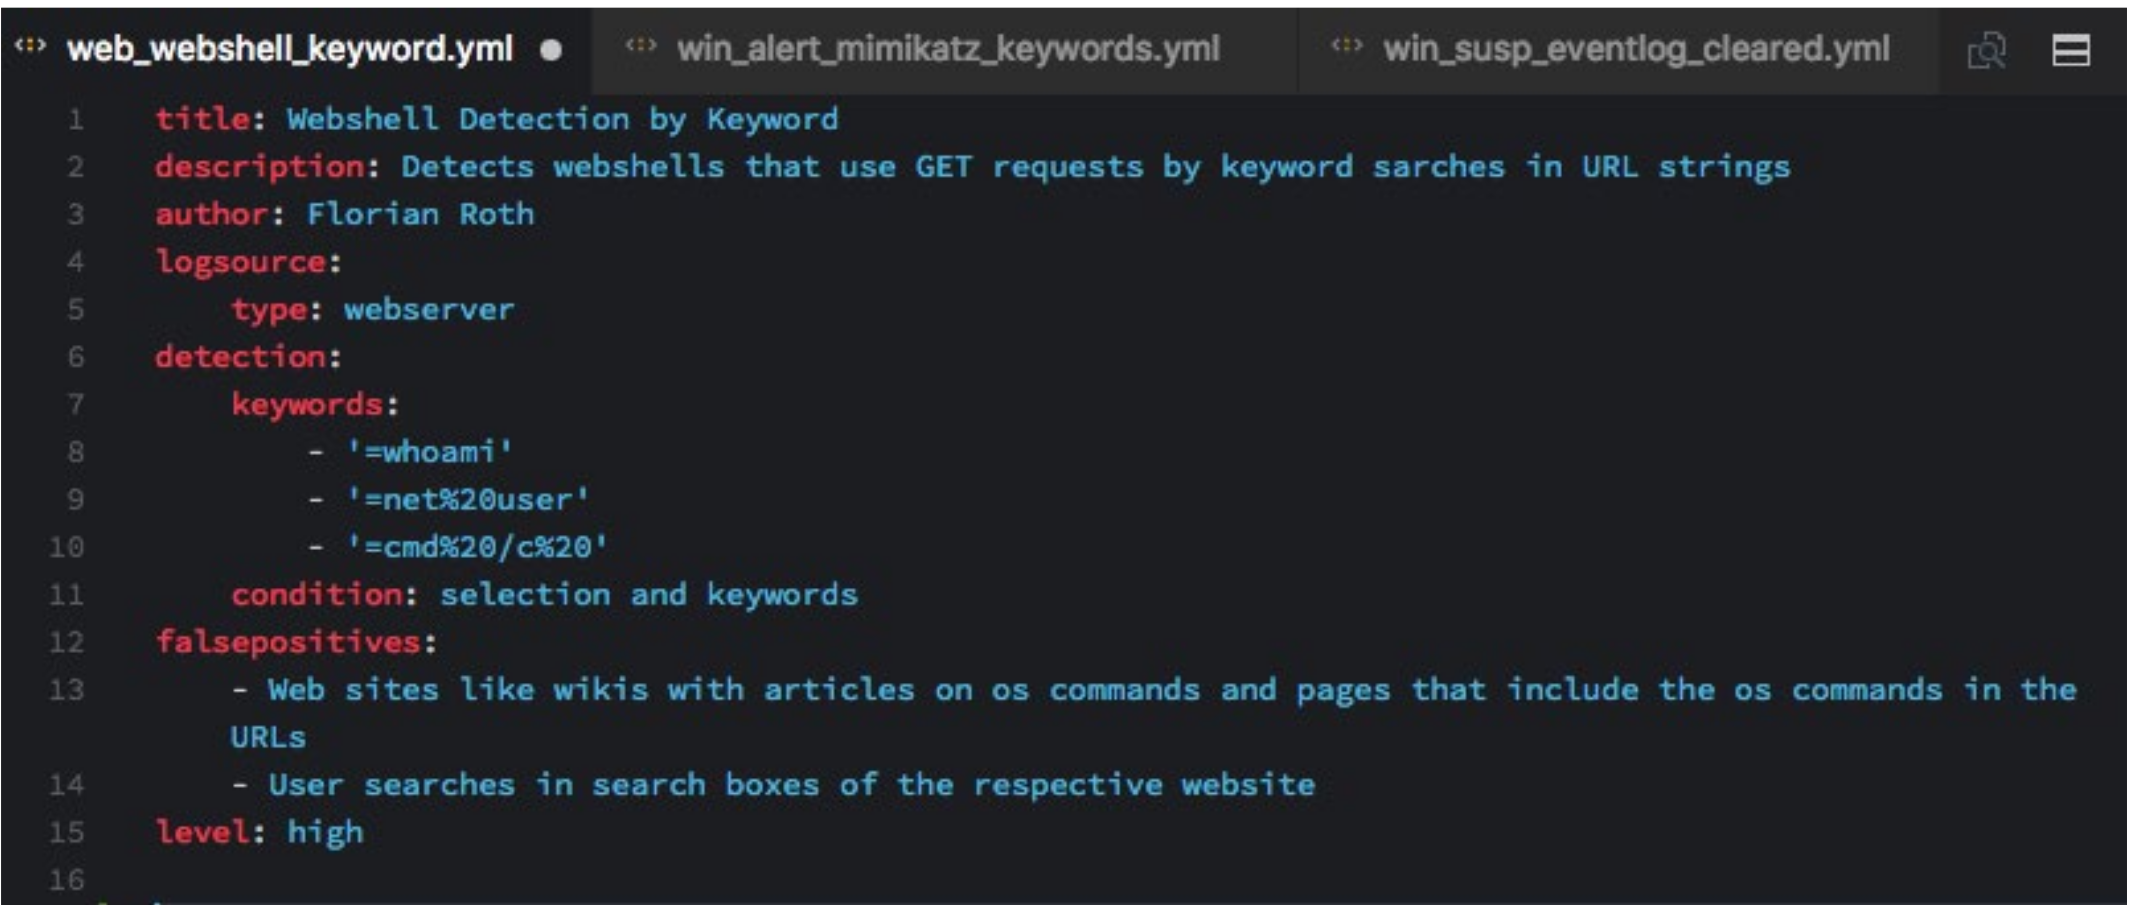
\includegraphics[width=\textwidth]{resources/12-sigma-detection-3.png}
\end{center}

\begin{center}
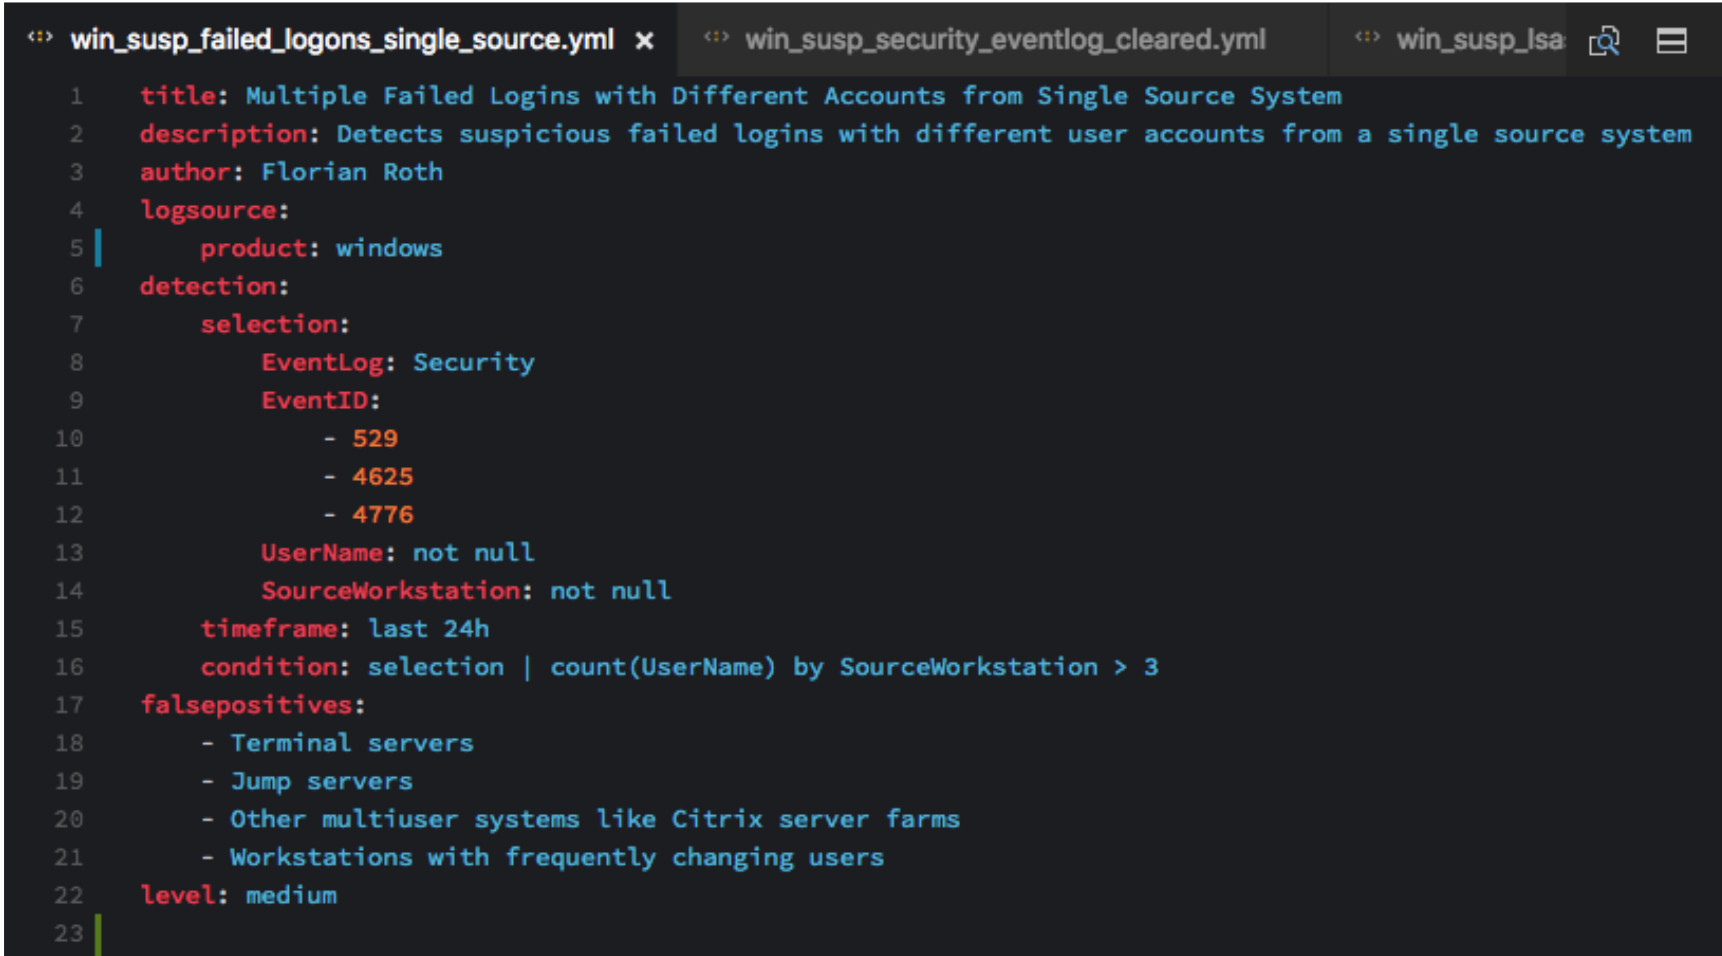
\includegraphics[width=\textwidth]{resources/12-sigma-detection-4.png}
\end{center}

\subsection{Forensic Readiness}
\begin{quotation}
  Be ready for the incident!
\end{quotation}

According to Forensics Readiness Guidelines (NICS, 2011)

Forensic Readiness is having an appropriate level of capability in order to be able to preserve, collect, protect and analyze digital evidence so that this evidence can be used effectively: in any legal matters; in security investigations; in disciplinary proceeding; in an employment tribunal; or in a court of law.

In other words: “Make sure you can correlate events from different it systems in a cascaded multi- tier and micro-service architecture”.

\subsubsection{Web Forensic Readiness}
Forensic Readiness with \textbf{UniqueID} == \textbf{RequestID}
\begin{center}
  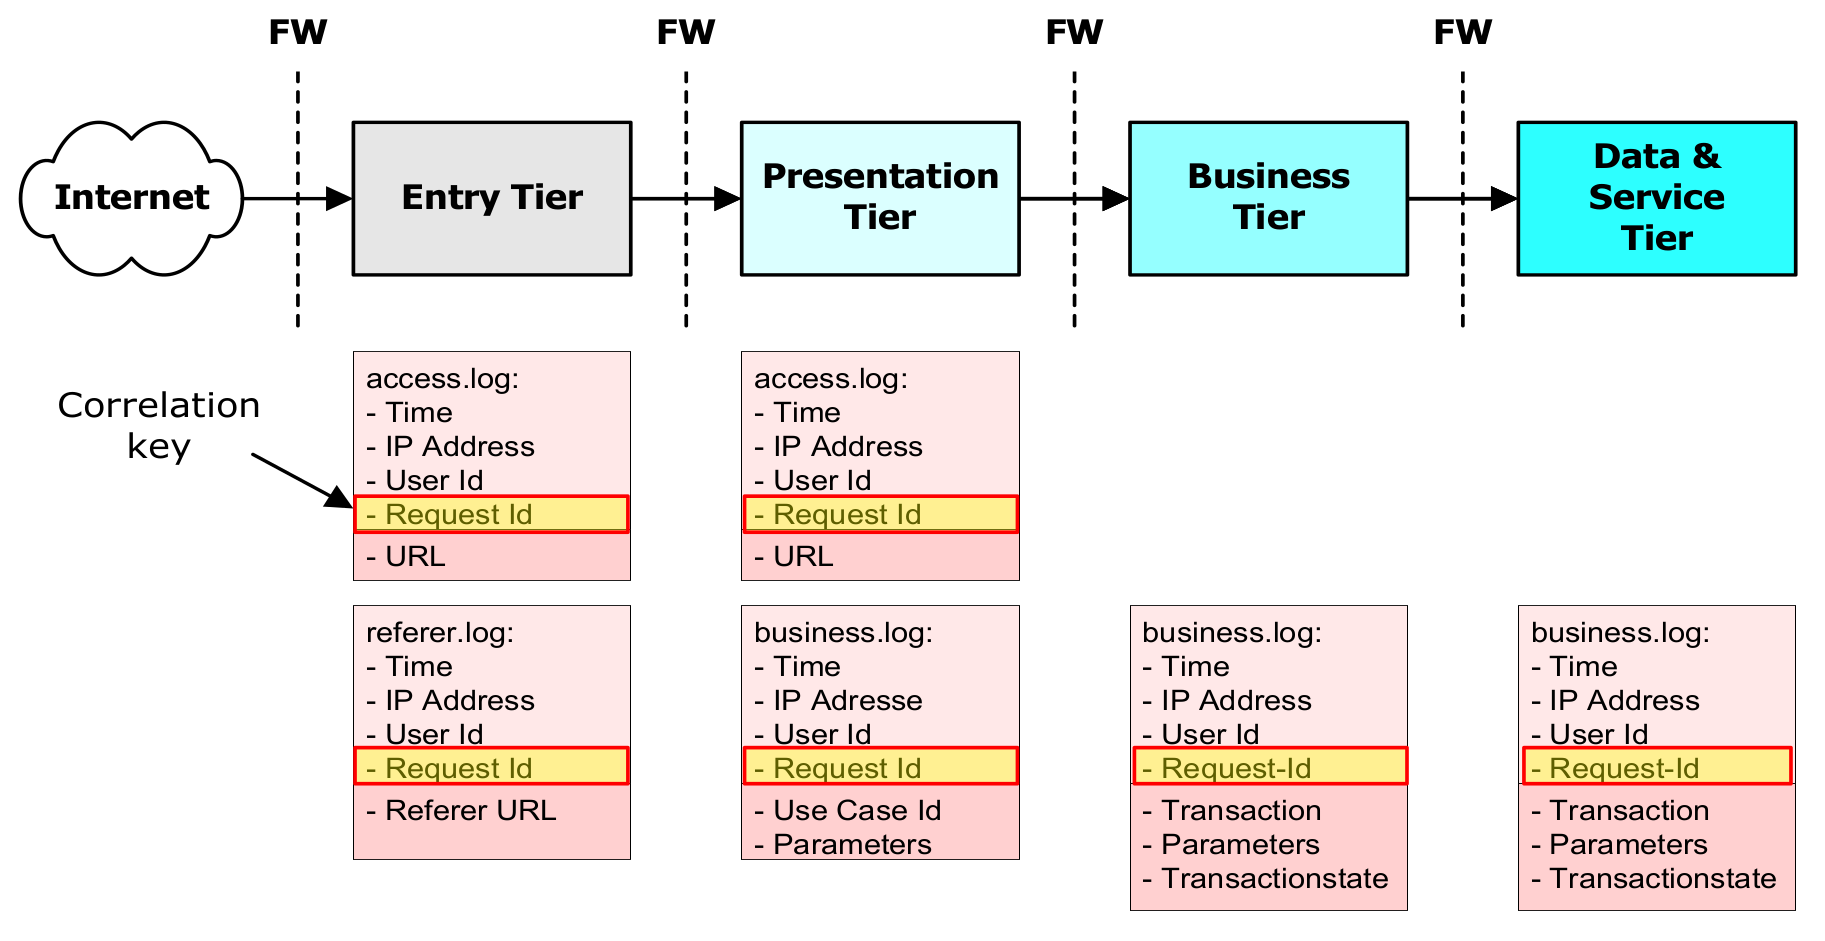
\includegraphics[width=\textwidth]{resources/12-forensic-readiness-1.png}
\end{center}

\subsubsection{Add Unique-ID to Requests}
\textbf{mod\_headers}

%\begin{center}
\begin{table}[h]
  \centering
  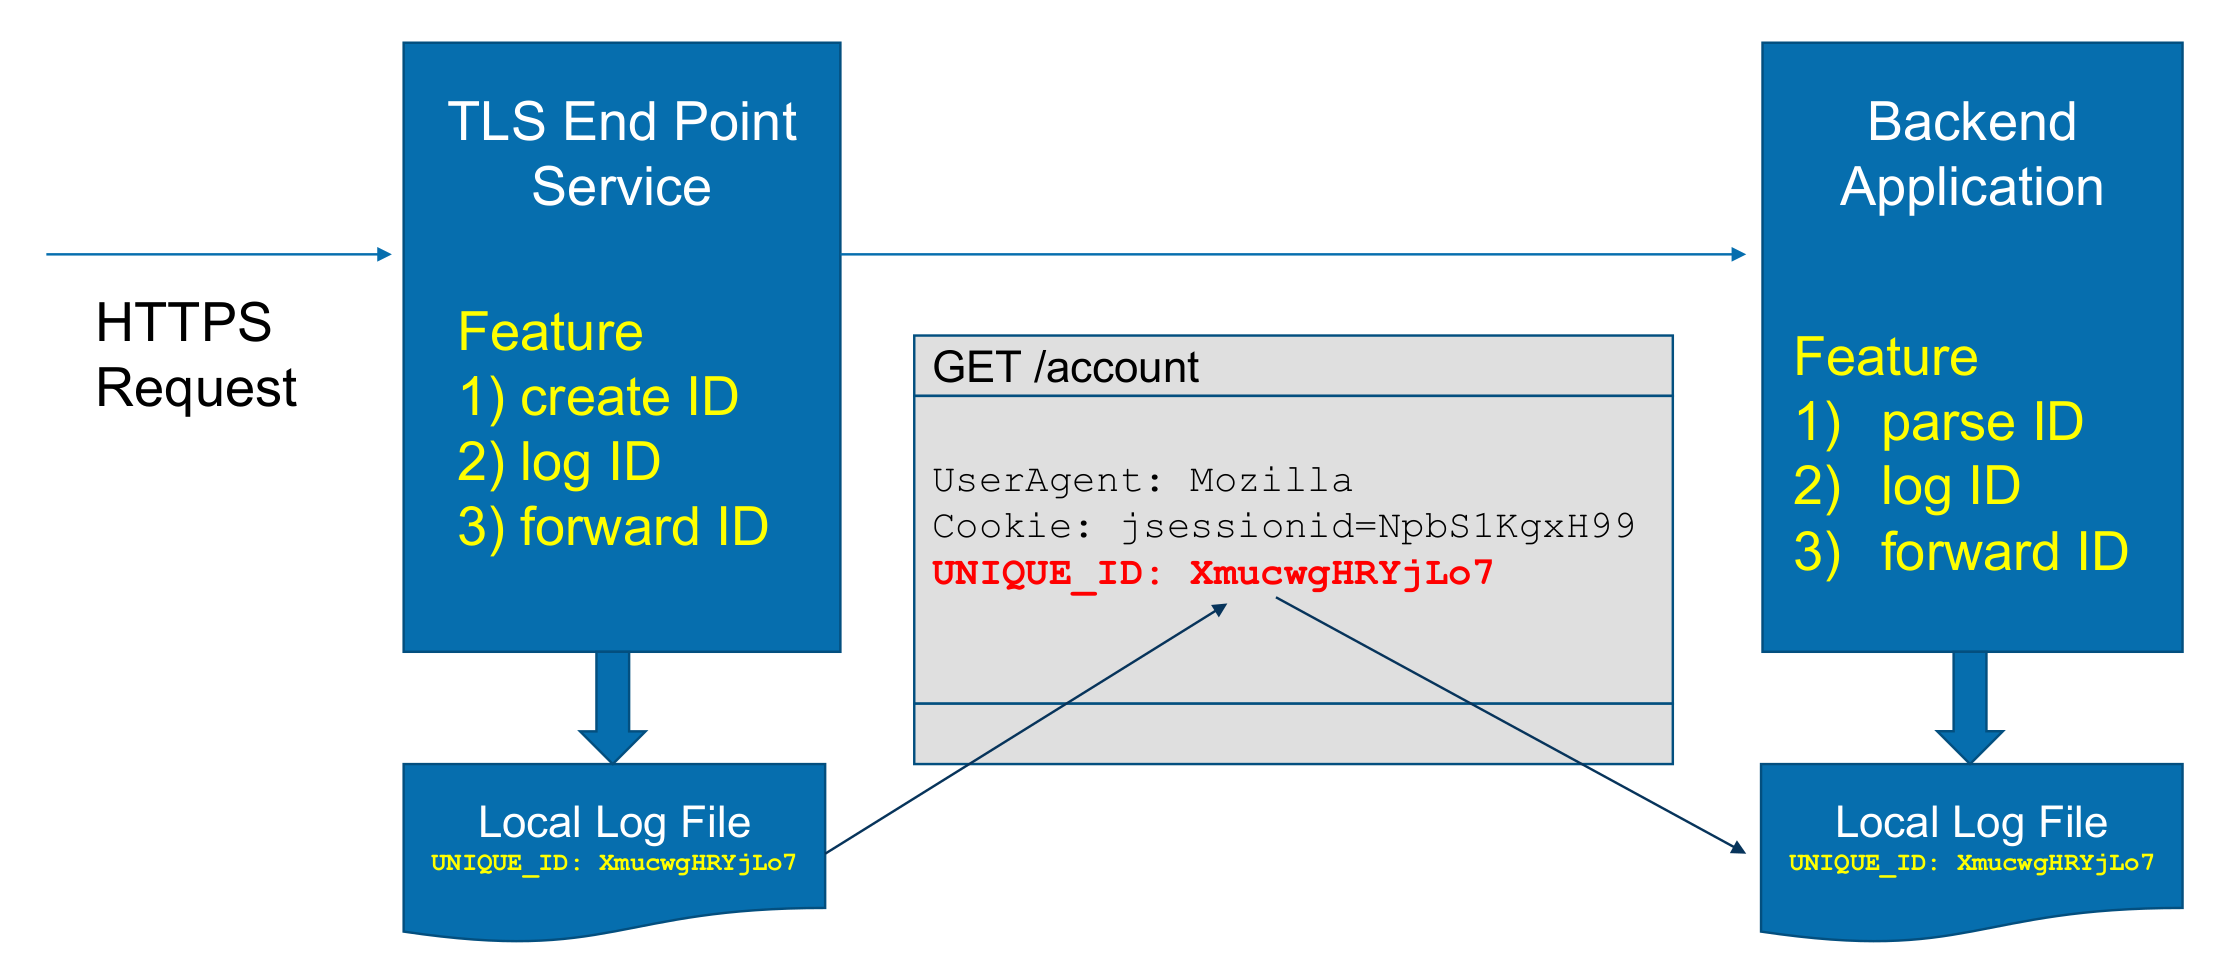
\includegraphics[width=\textwidth]{resources/12-unique-id-request-header.png}
  \caption{Unique-ID Request Header in Backend Application}
\end{table}
%\end{center}

RequestHeader append UNIQUE\_ID \%\{UNIQUE\_ID\}'
\begin{table}[h]
  \centering
  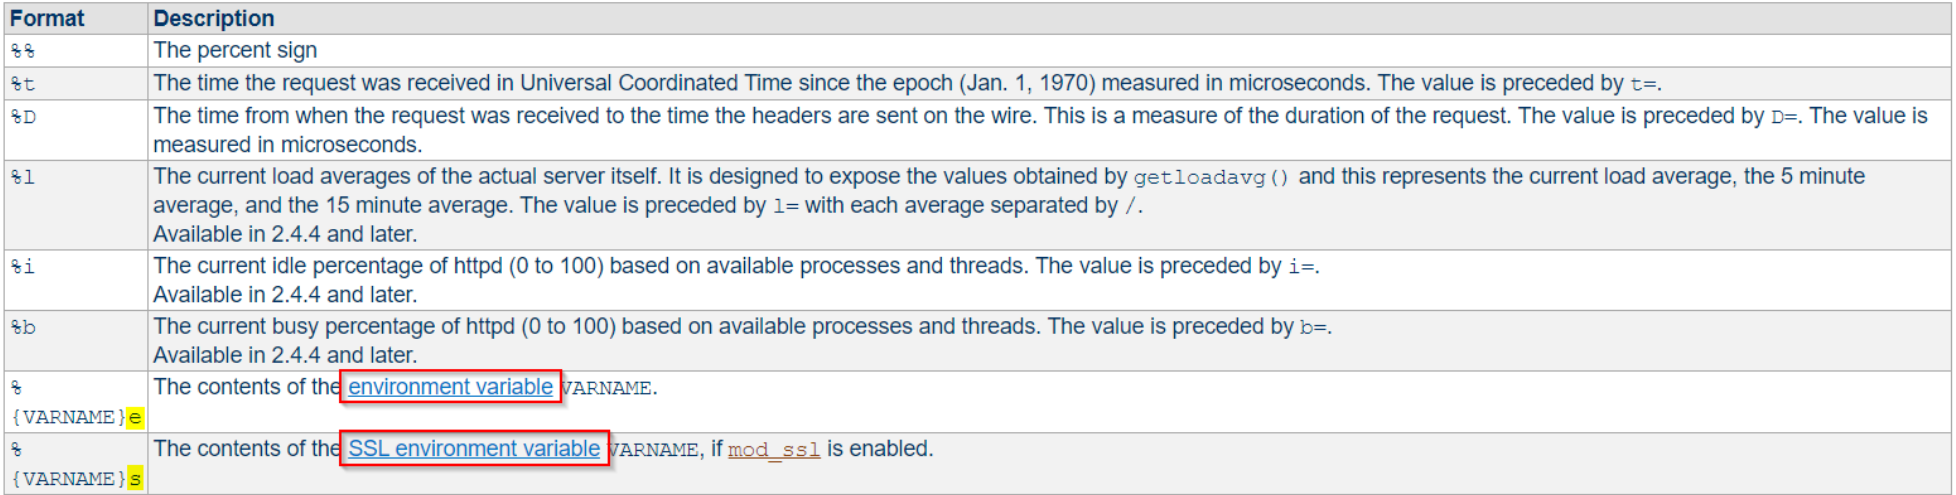
\includegraphics[width=\textwidth]{resources/12-unique-id-request-header-2.png}
  \caption{Adding Headers to Request  - mod\_headers}
\end{table}

\begin{table}[h]
  \centering
  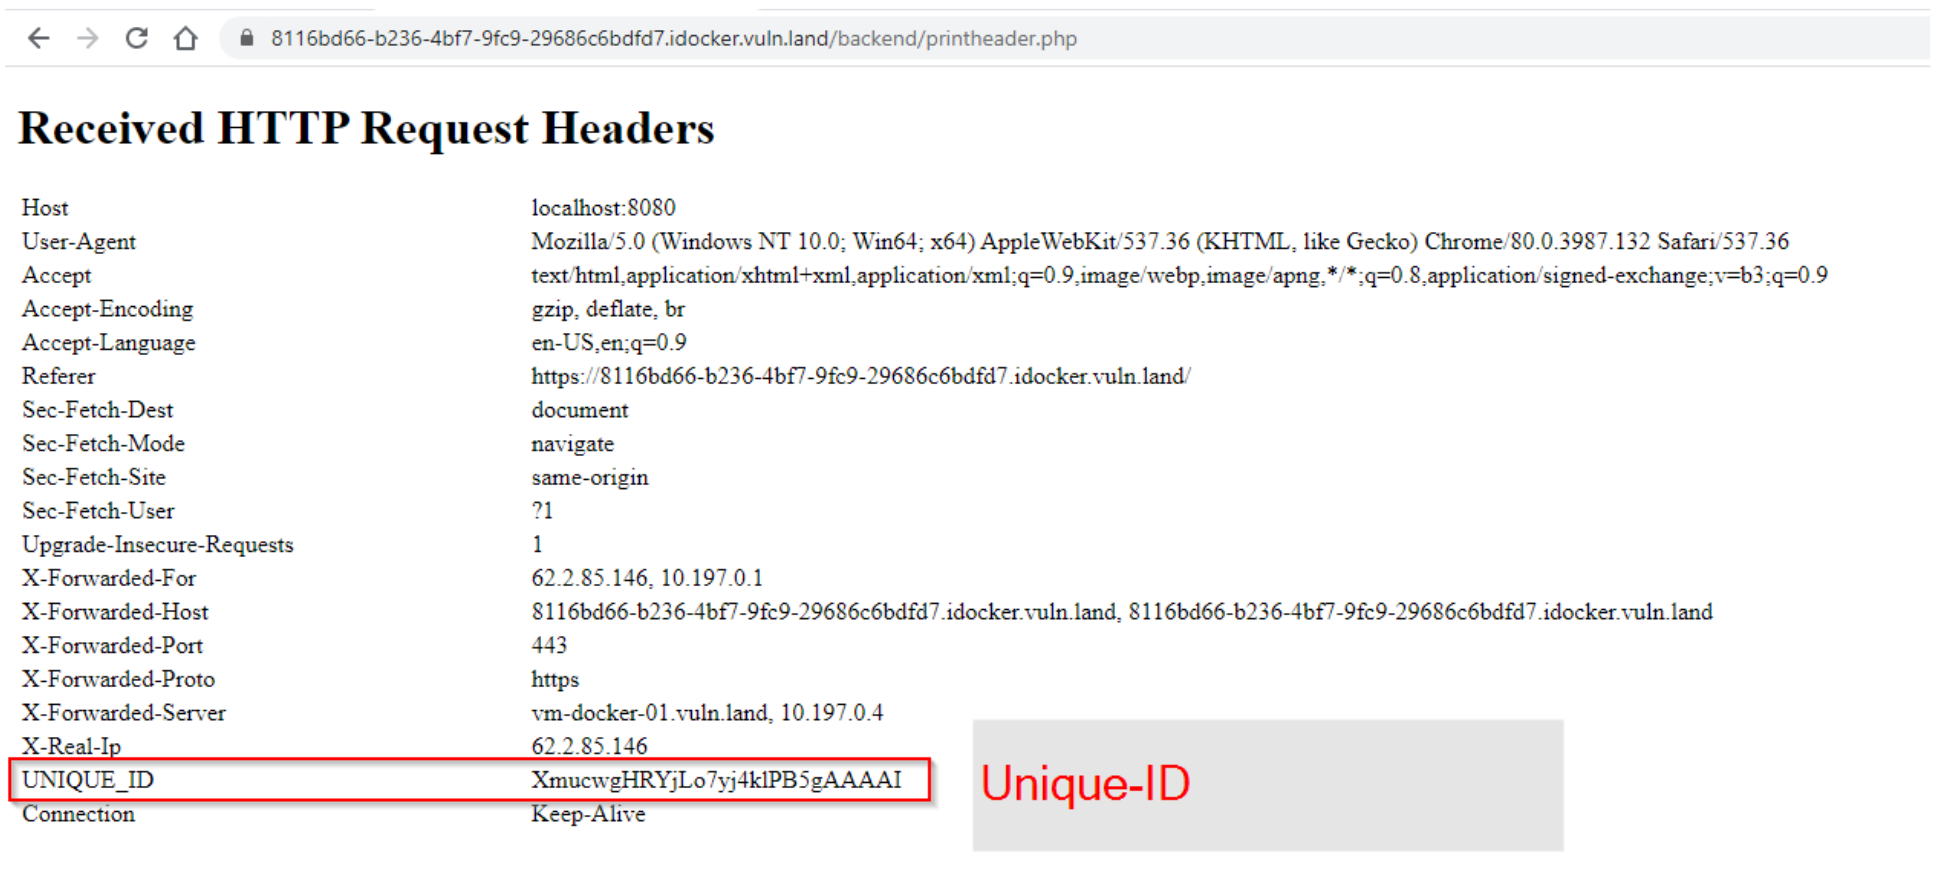
\includegraphics[width=\textwidth]{resources/12-unique-id-request-header-3.png}
  \caption{Adding Headers to Request  - example}
\end{table}

\subsection{Add Unique-ID to Logfile}

Apache Web Server: two Types of Log Configurations

\begin{table}[h]
  \centering
  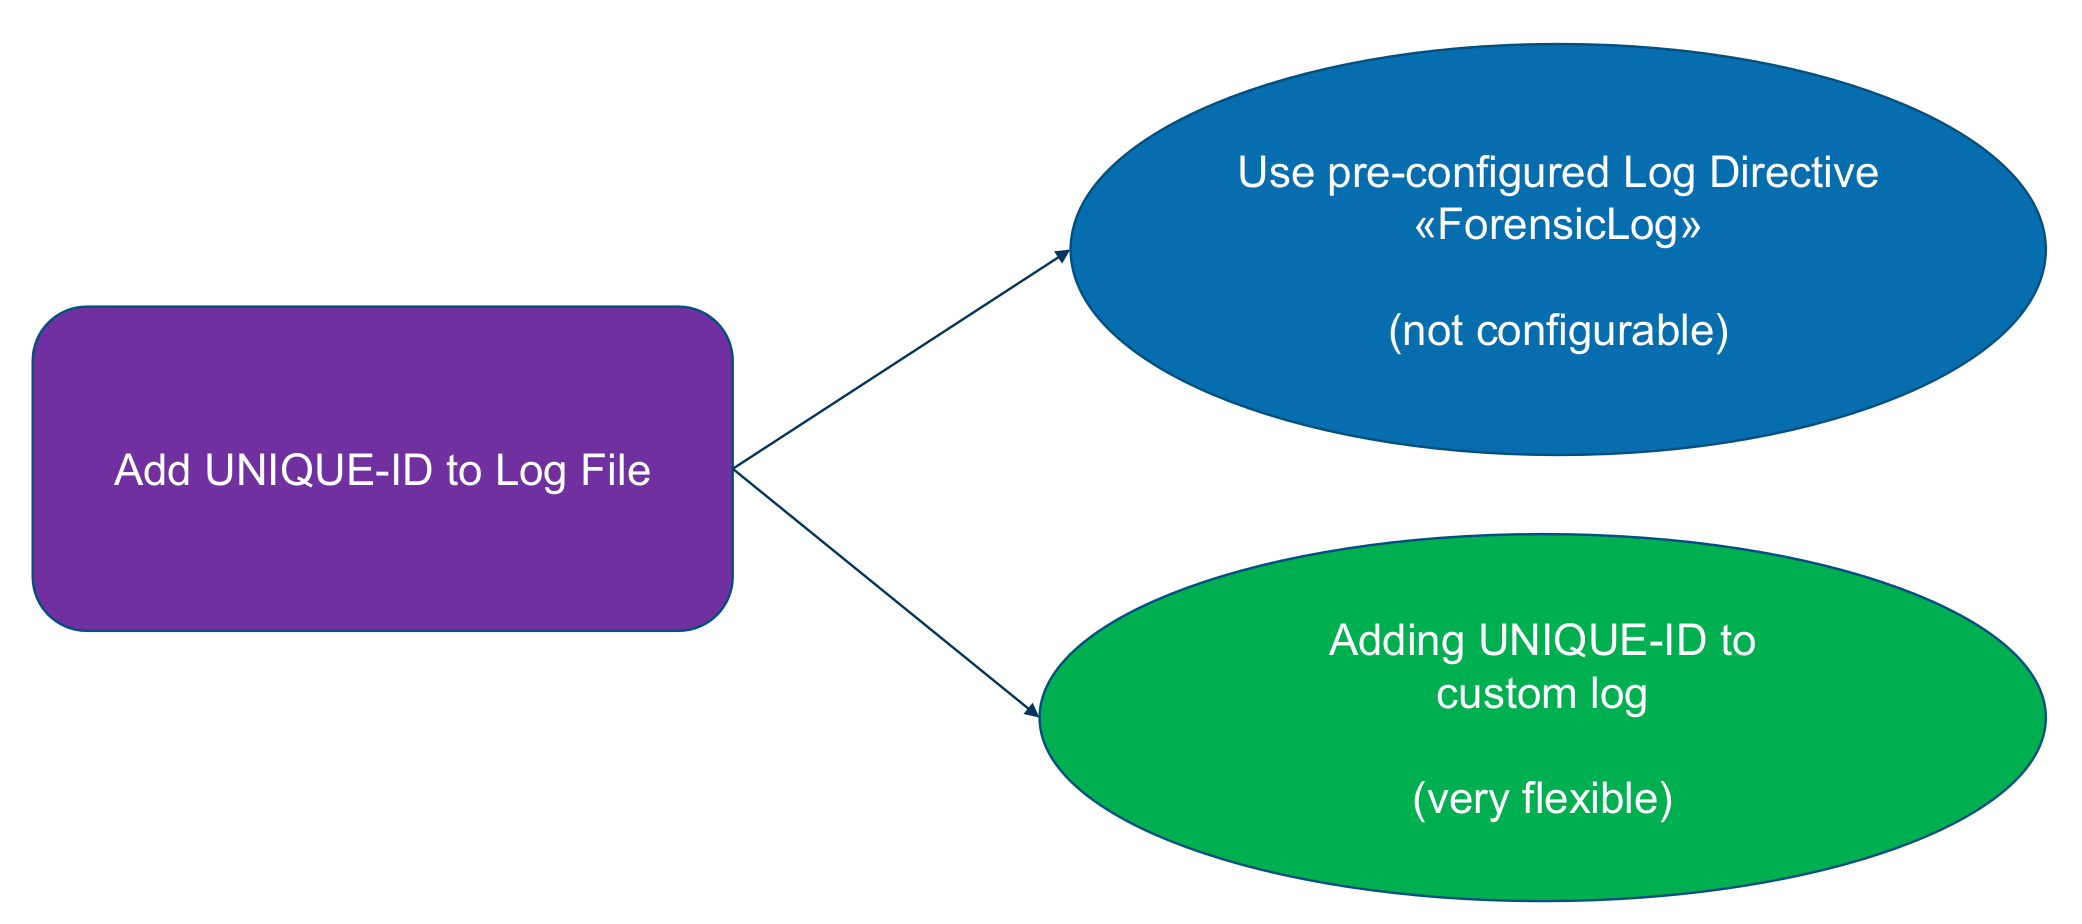
\includegraphics[width=\textwidth]{resources/12-apache-add-unique-id-to-log.png}
  \caption{Apache Logging - Unique ID}
\end{table}

\begin{table}[h]
  \centering
  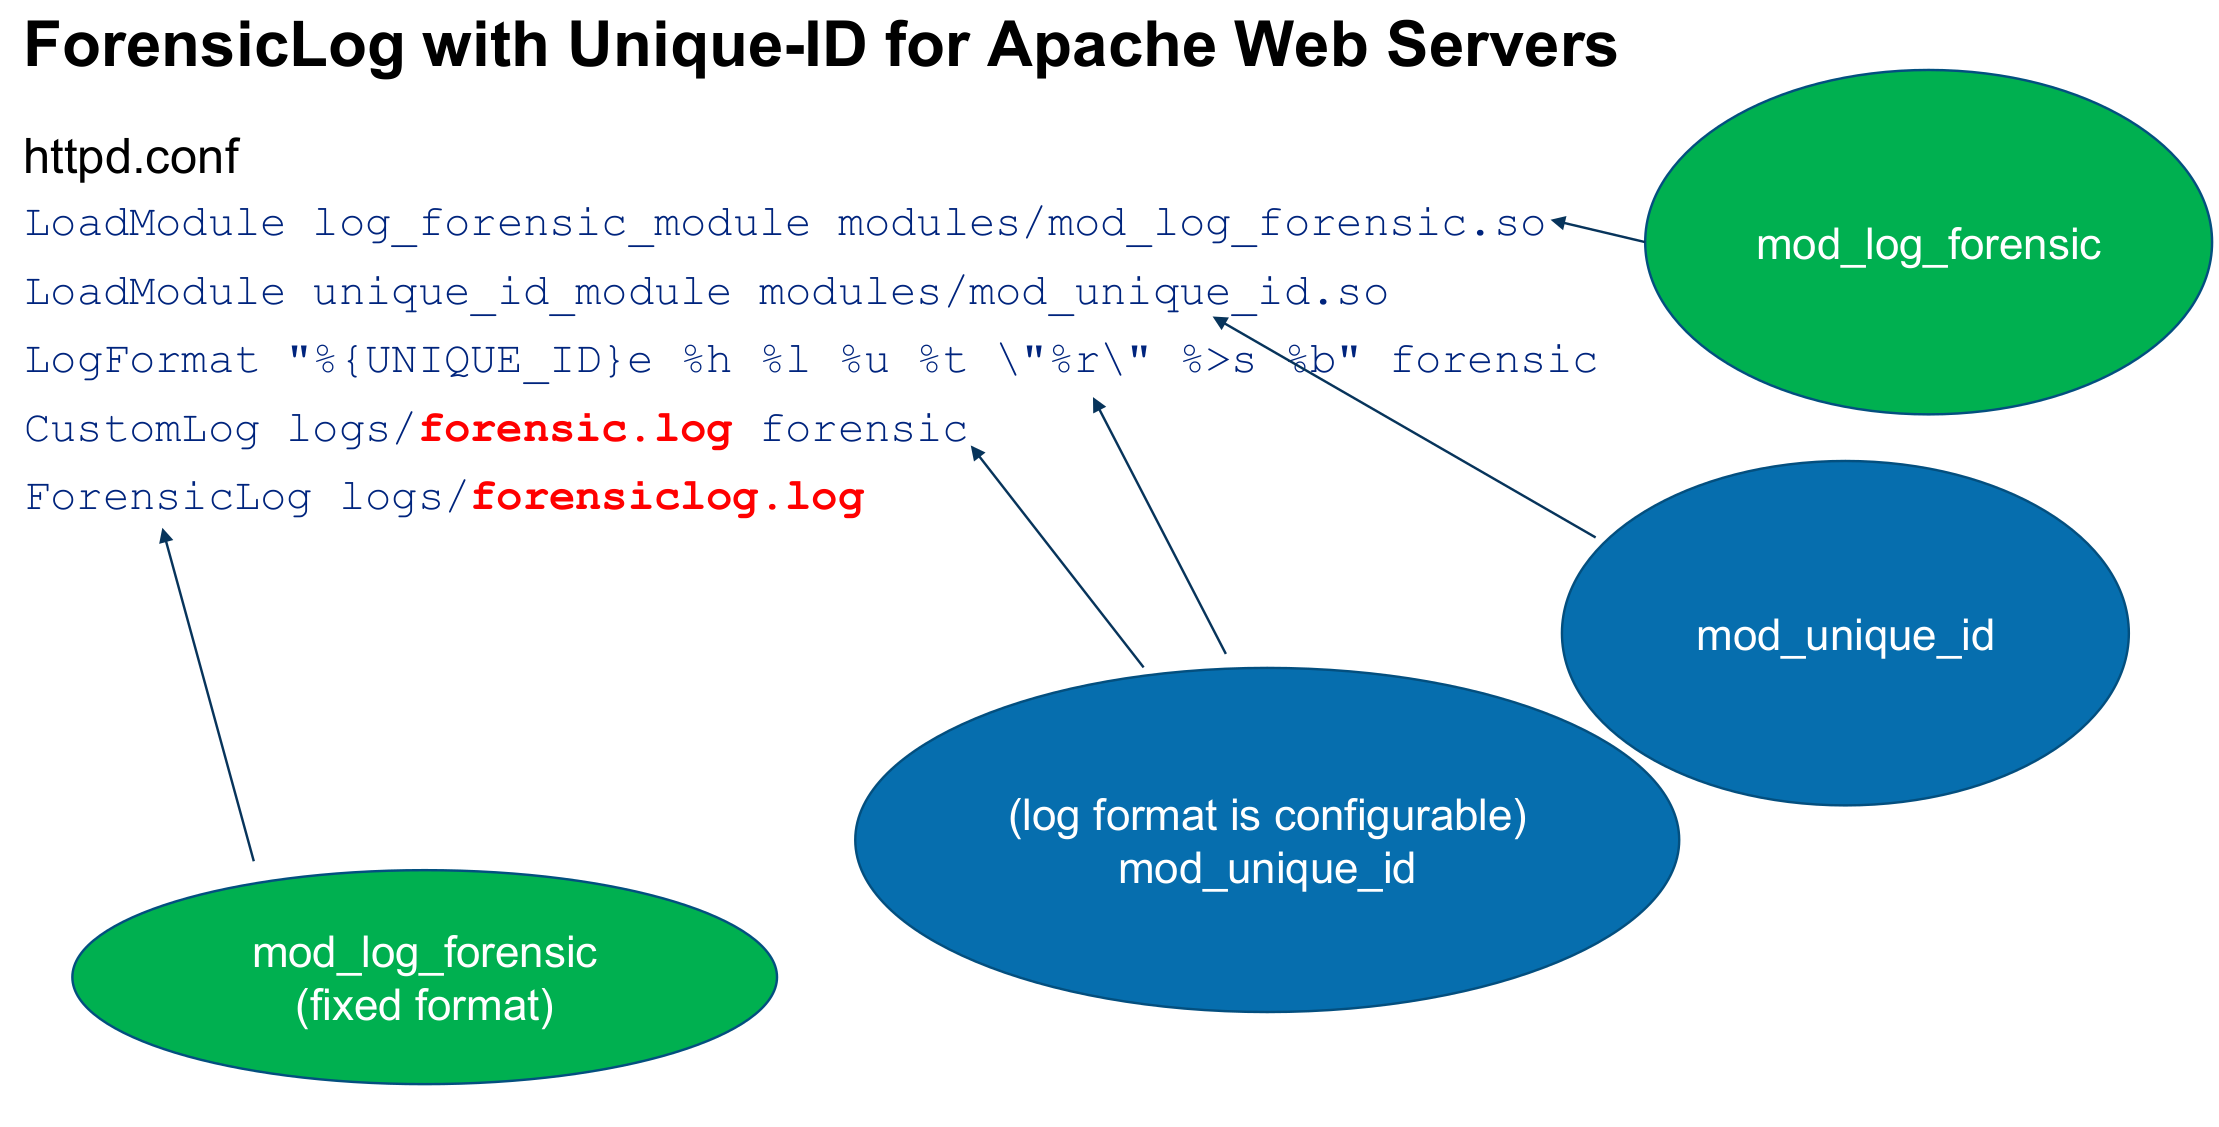
\includegraphics[width=\textwidth]{resources/12-apache-add-unique-id-to-log-2.png}
  \caption{Apache Logging - Unique ID ForensicLog}
\end{table}

\subsubsection{Static ForensicLog}

\begin{table}[h]
  \centering
  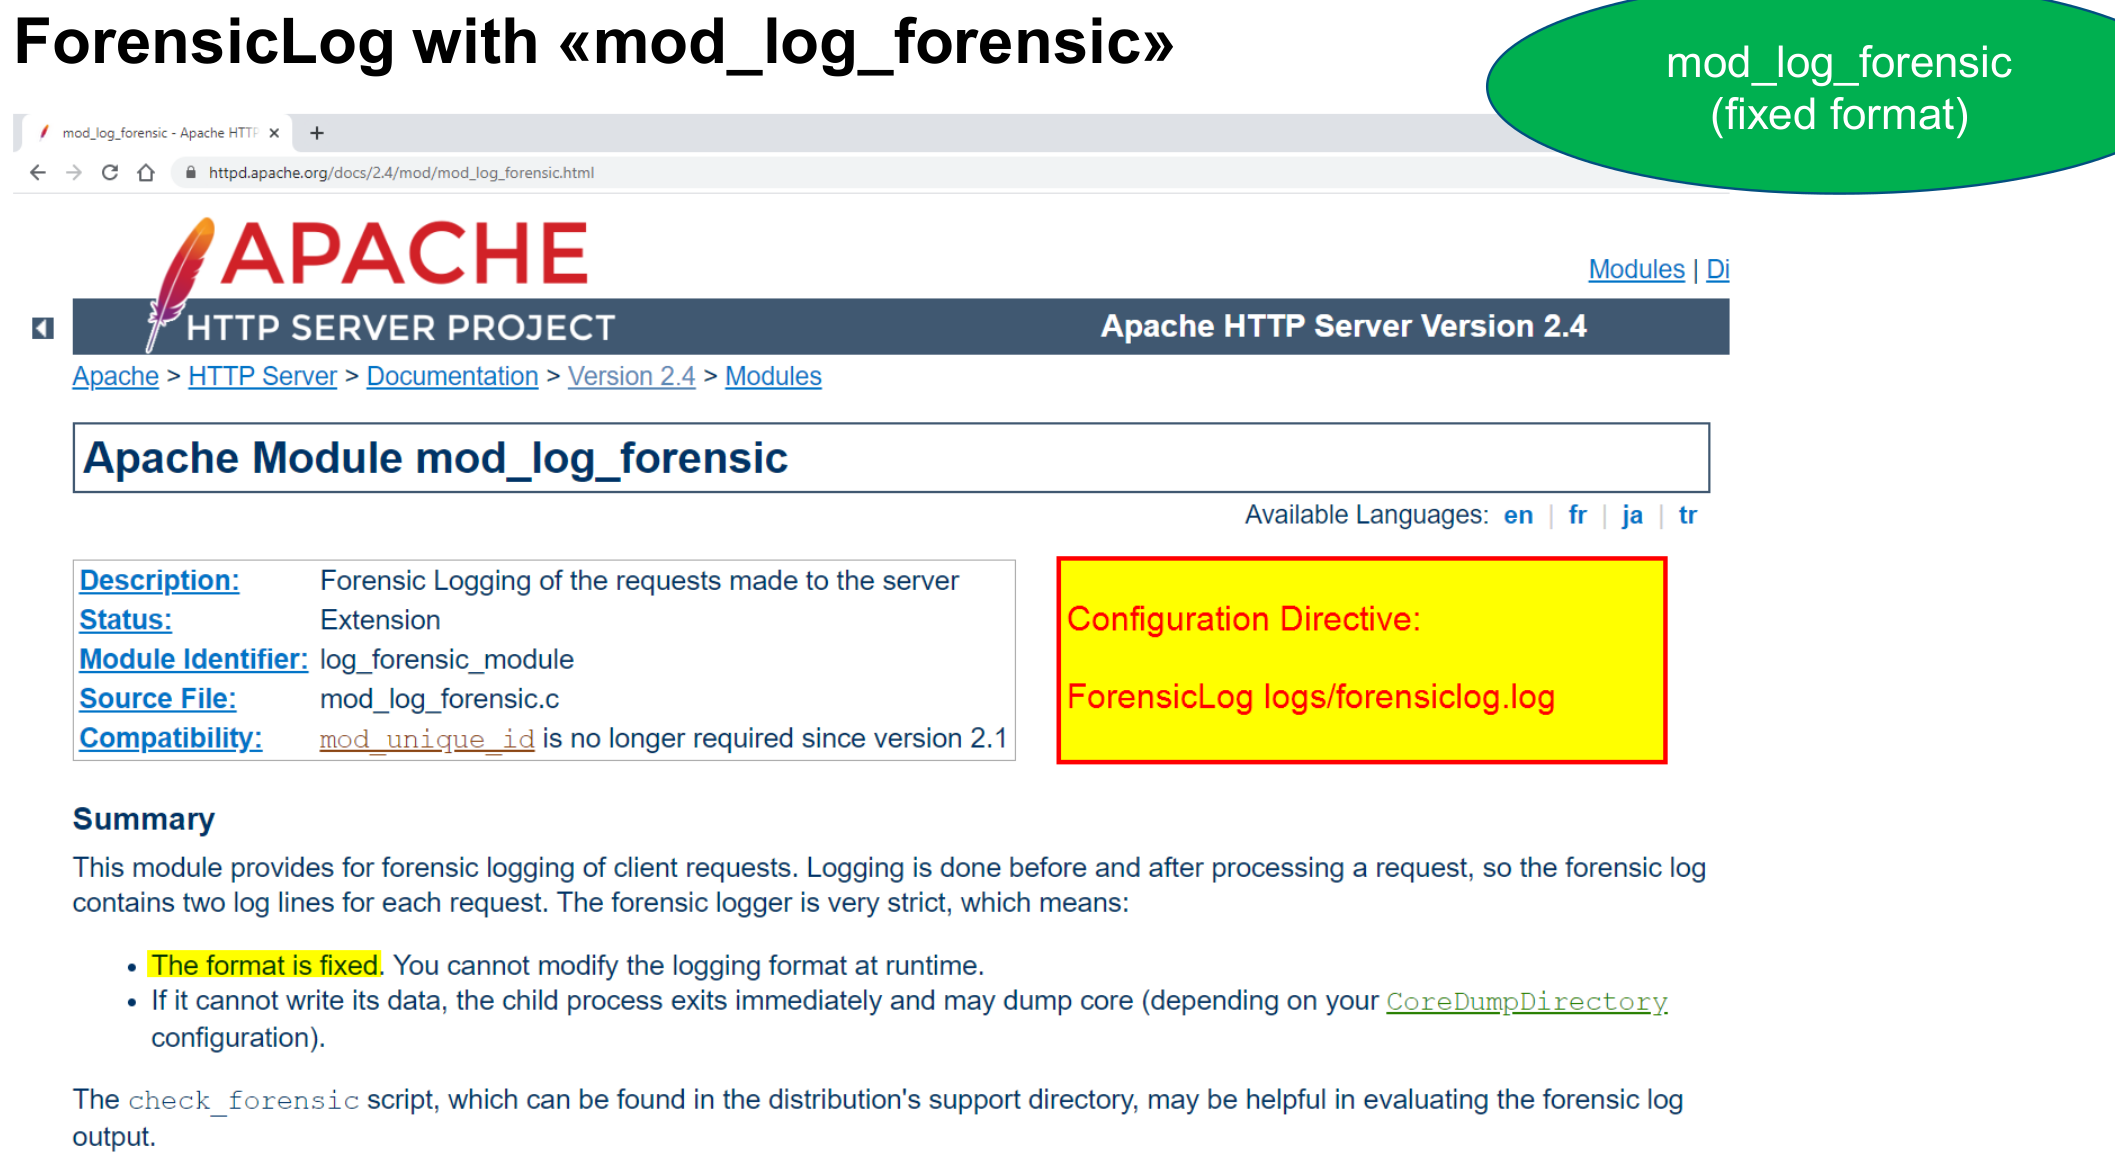
\includegraphics[width=\textwidth]{resources/12-apache-forensic-log.png}
  \caption{Apache Logging - ForensicLog with mod\_log\_forensic}
\end{table}

\begin{table}[h]
  \centering
  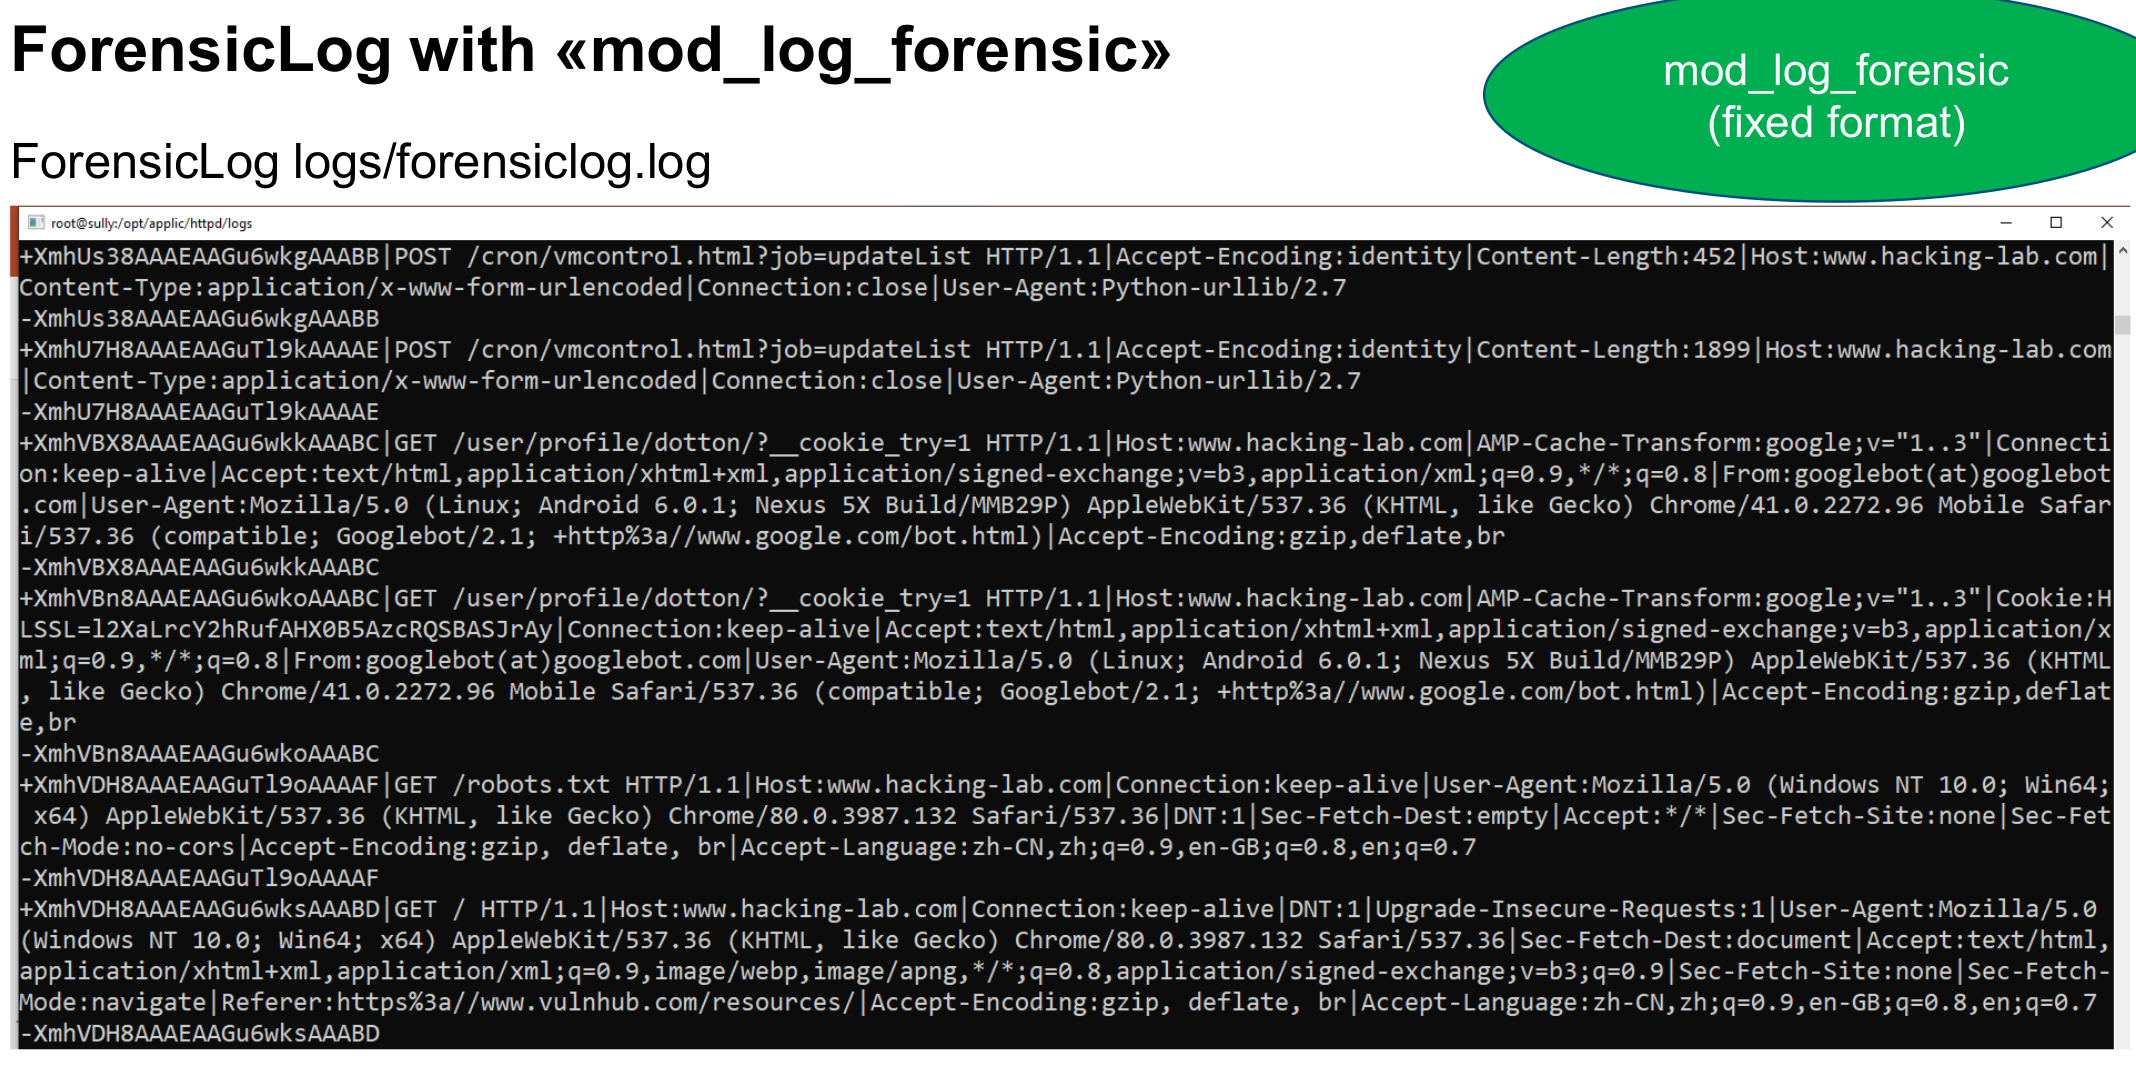
\includegraphics[width=\textwidth]{resources/12-apache-forensic-log-2.png}
  \caption{Apache Logging - ForensicLog with mod\_log\_forensic example}
\end{table}

\subsubsection{Custom Log mod\_log\_config}

\begin{table}[h]
  \centering
  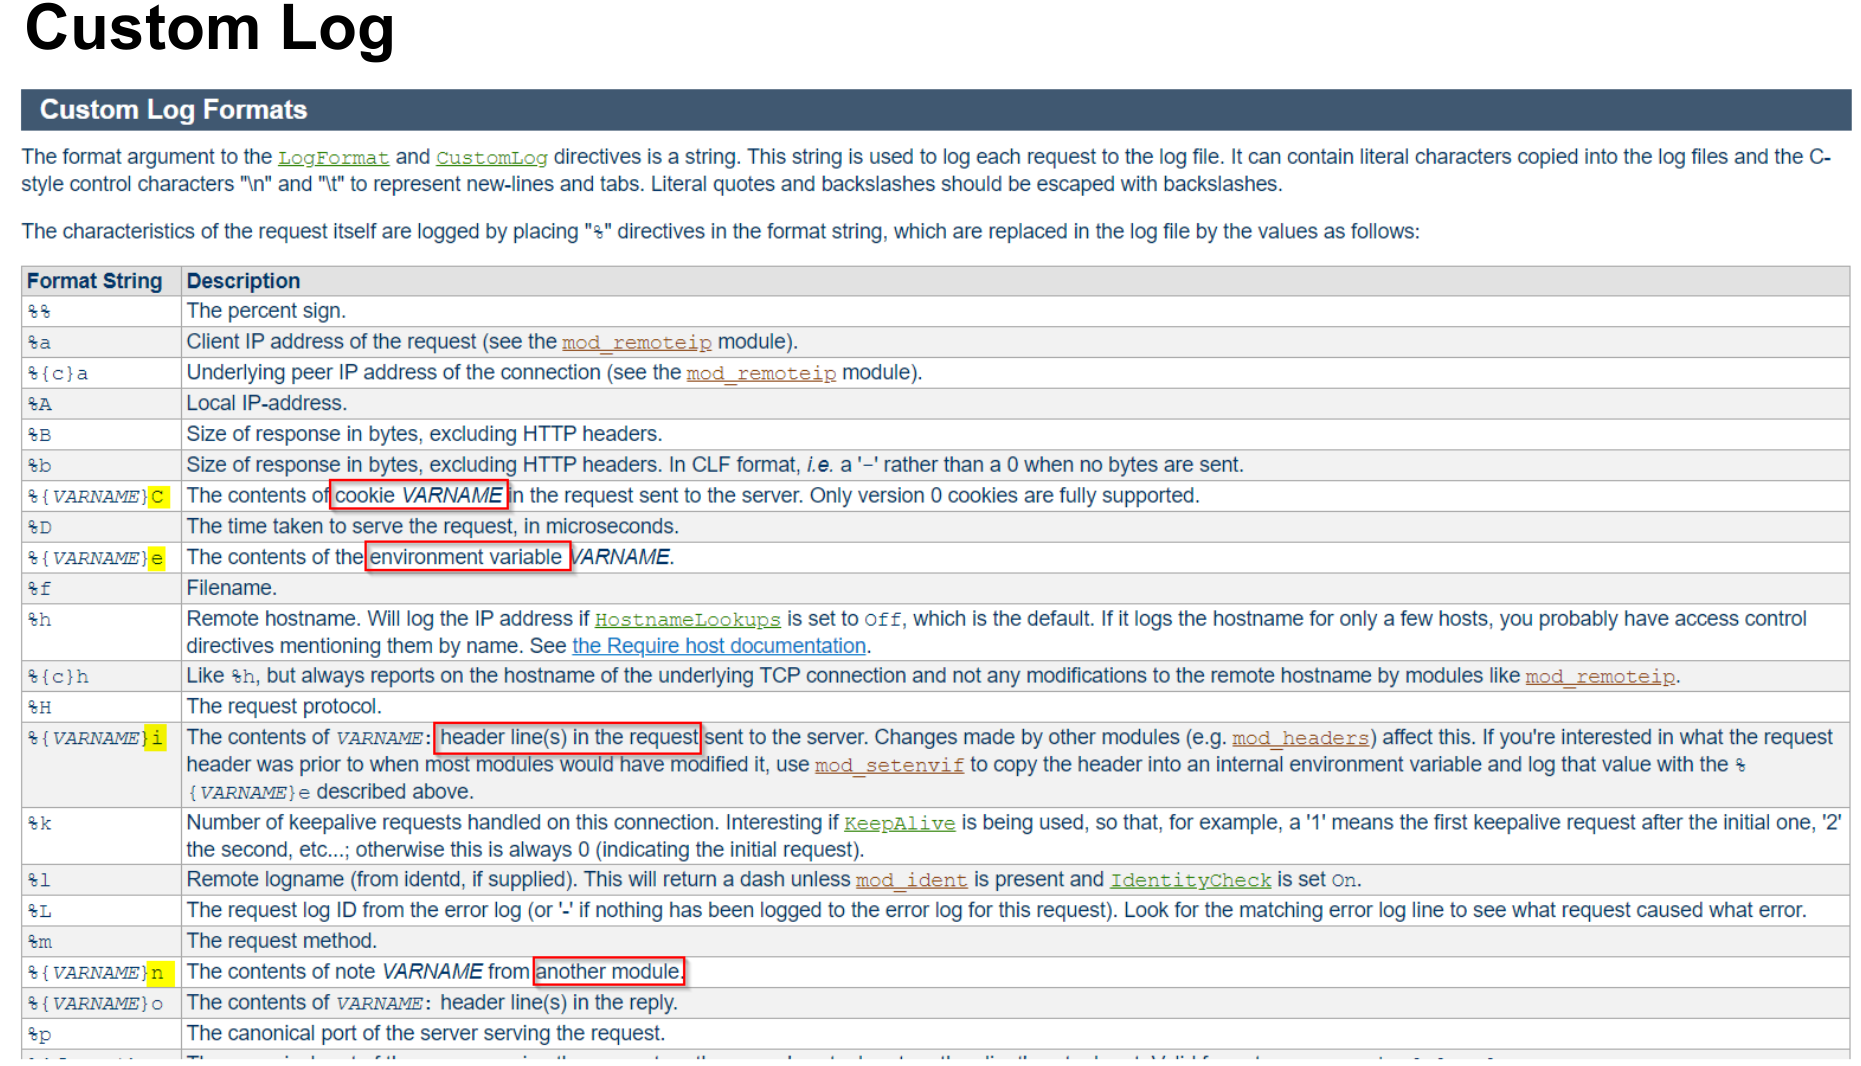
\includegraphics[width=\textwidth]{resources/12-apache-custom-log.png}
  \caption{Apache Logging - custom log}
\end{table}

LogFormat "\%\{UNIQUE\_ID\}e \%h \%l \%u \%t \\"\%r\\" \%\>s \%b \\"\%\{Referer\}i\\" \\"\%\{User\-Agent\}i\\"" forensic CustomLog logs/forensic.log forensic

\begin{table}[h]
  \centering
  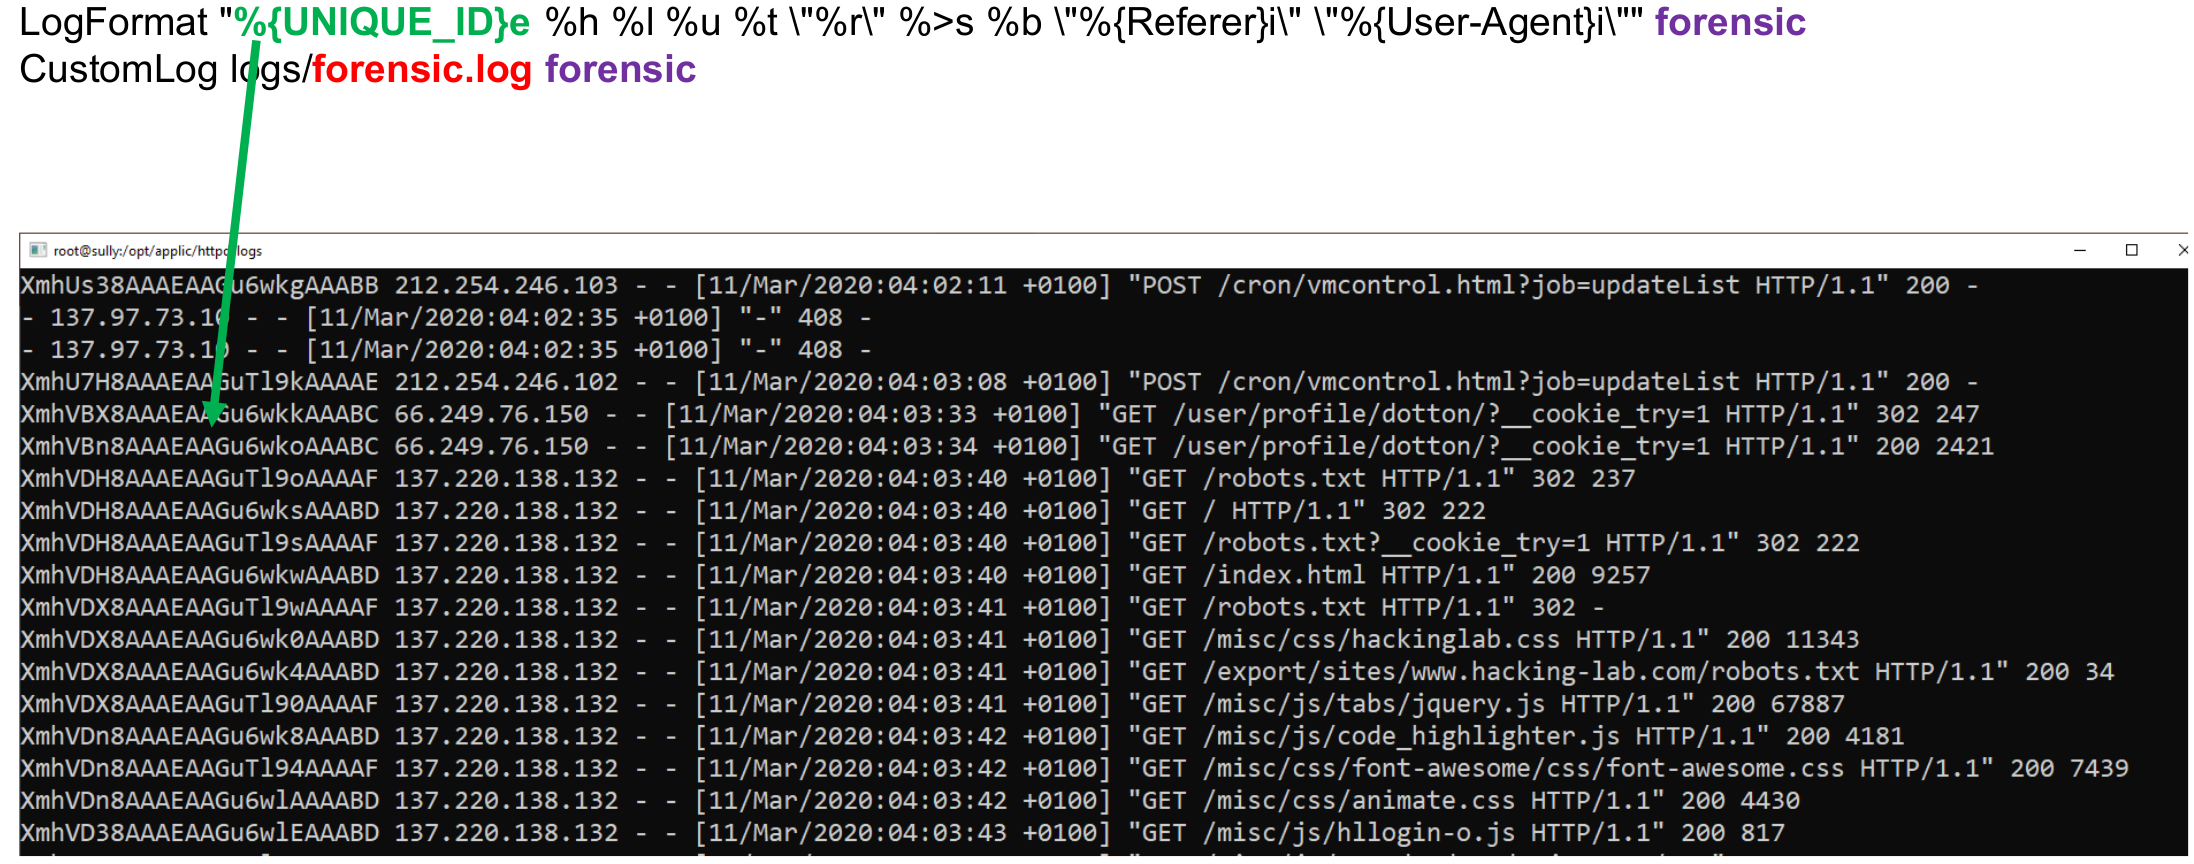
\includegraphics[width=\textwidth]{resources/12-apache-custom-log-2.png}
  \caption{Apache Logging - custom log example}
\end{table}

\textbf{What is the benefit of the Unique-ID?}
\begin{itemize}
  \item Correlation of events among multi-tier and micro-service architectures
  \item Because a timestamp is not sufficient!!!!
  \item First server (internet facing) that should generate the unique-id and add the id to the own log files. Furthermore, the unque-id should be handed over to backend services, usually by adding a special header. The backend services should parse the unique-id and add it to the own logs. Furthermore, it should add the unique-id to any further server or instance. If this would be the case for all services – you can always find out what who, when, where something happended.
  \item Without the unique-id, companies are lost and must relay on timestamps
\end{itemize}

\subsection{Fraud Detection}
\subsubsection{Types of Phishing Attacks}
\begin{itemize}
  \item E-Banking Online Phishing Attacks
  \item E-Banking Attack Session Hijacking
  \item Man-in-the-Browser Attack
\end{itemize}

\begin{table}[h]
  \centering
  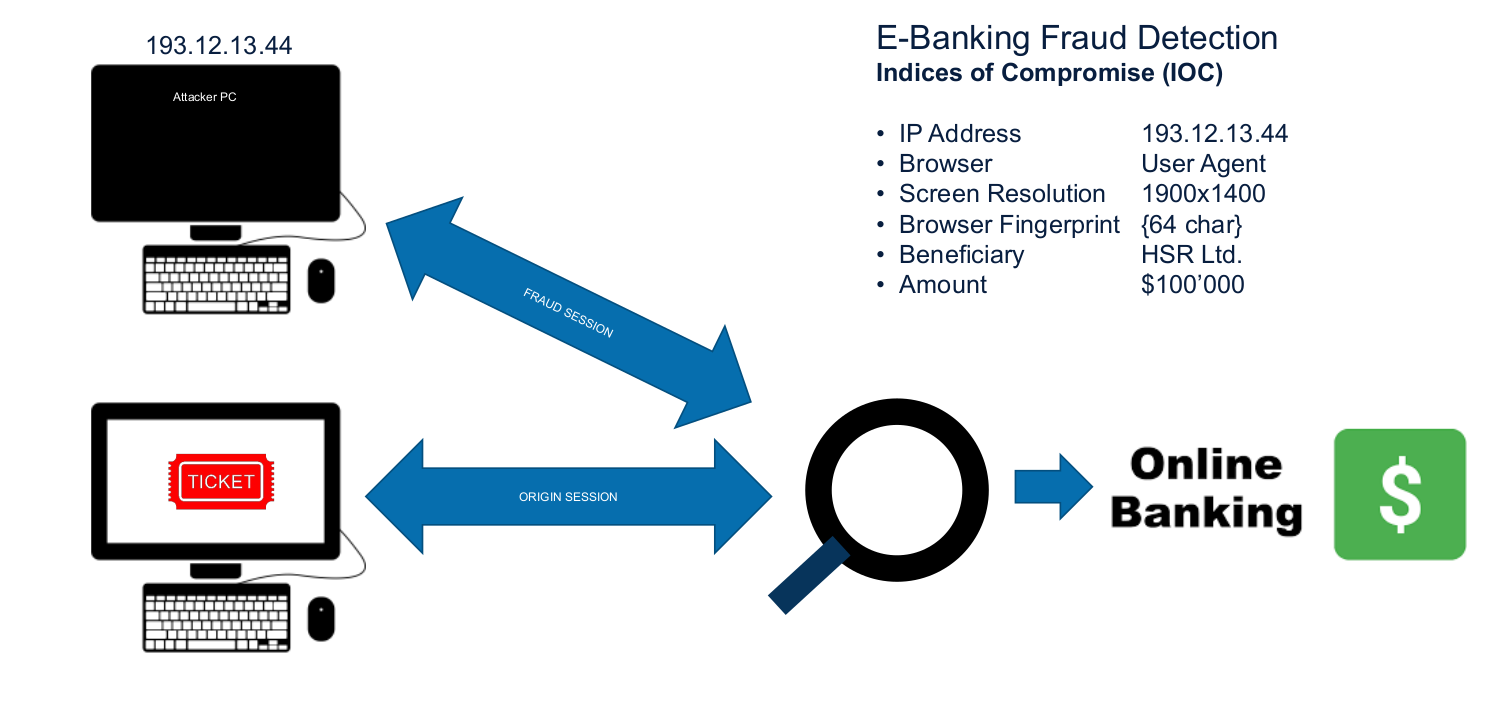
\includegraphics[width=\textwidth]{resources/12-frau-detection.png}
  \caption{Fraud Detection - E-Banking Online Phishing Attack}
\end{table}

\begin{table}[h]
  \centering
  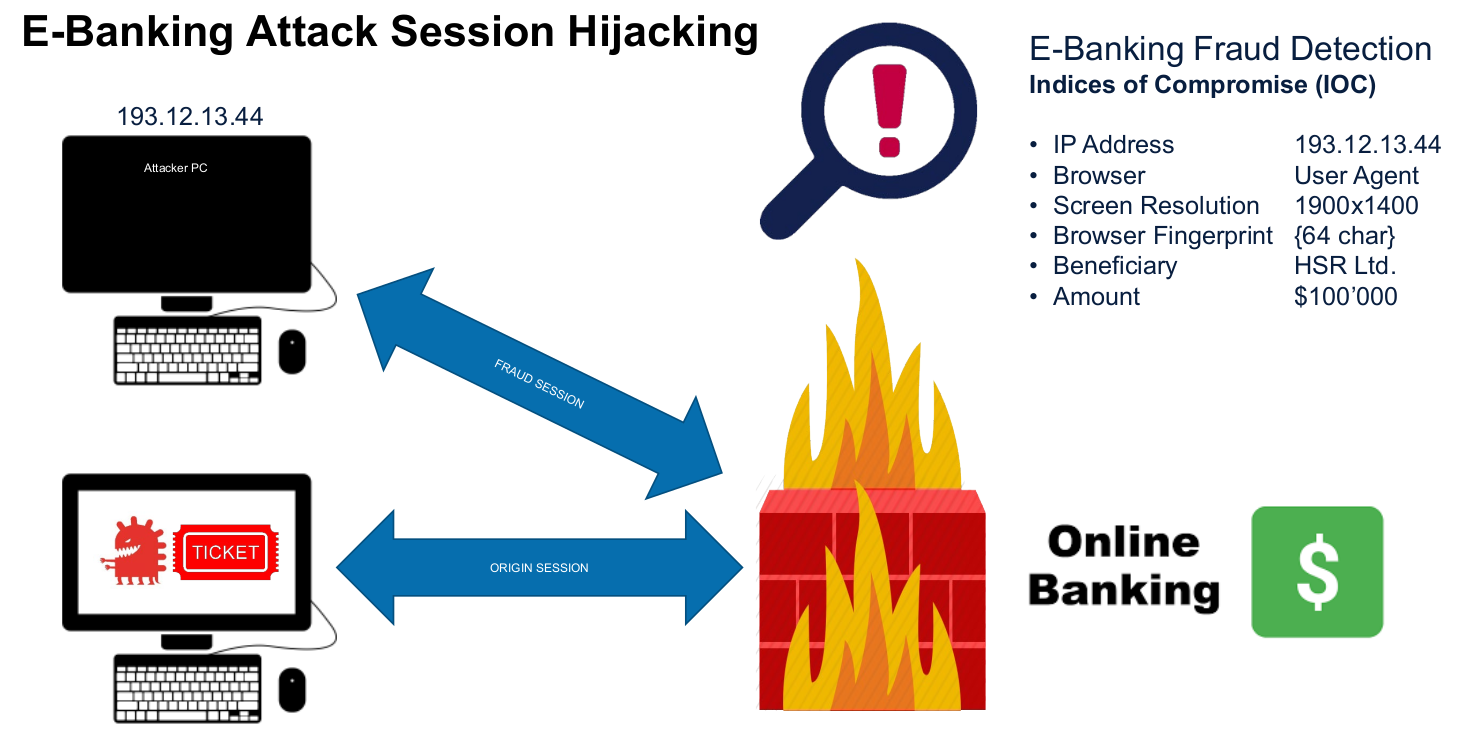
\includegraphics[width=\textwidth]{resources/12-fraud-detection-2.png}
  \caption{Fraud Detection - E-Banking Attack Session Hijacking}
\end{table}

\begin{table}[h]
  \centering
  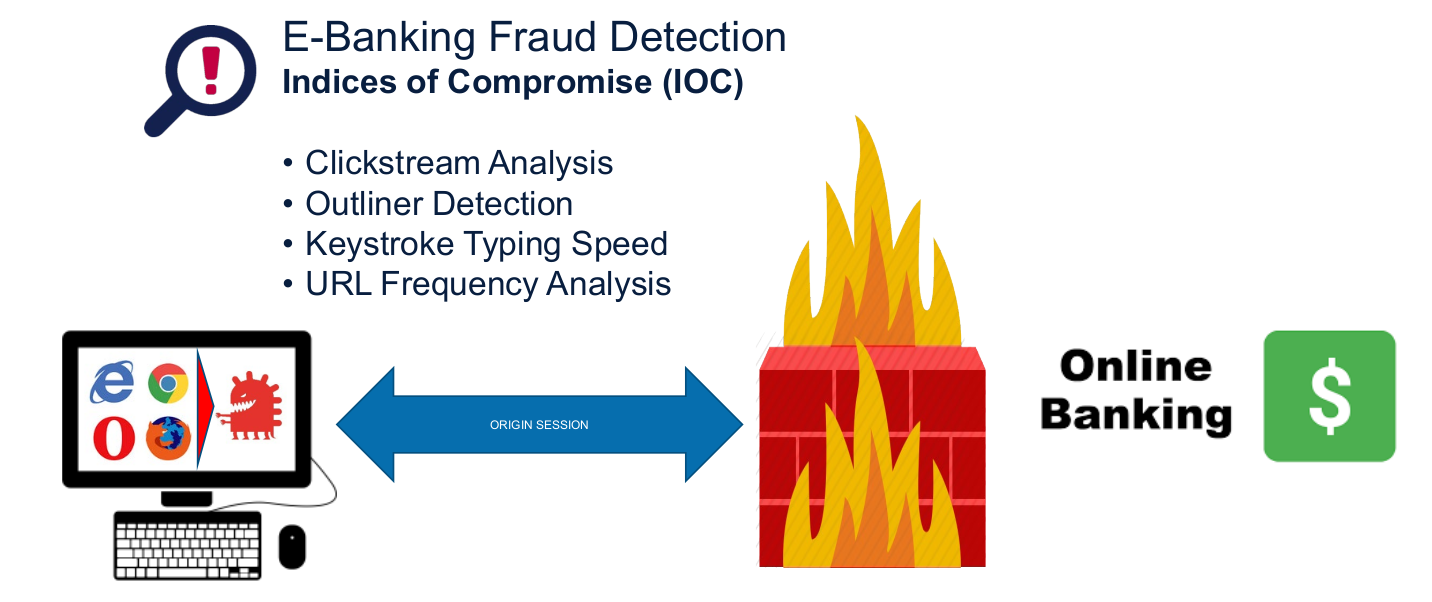
\includegraphics[width=\textwidth]{resources/12-fraud-detection-3.png}
  \caption{Fraud Detection - Man-in-the-Browser MitB}
\end{table}

\begin{table}[h]
  \centering
  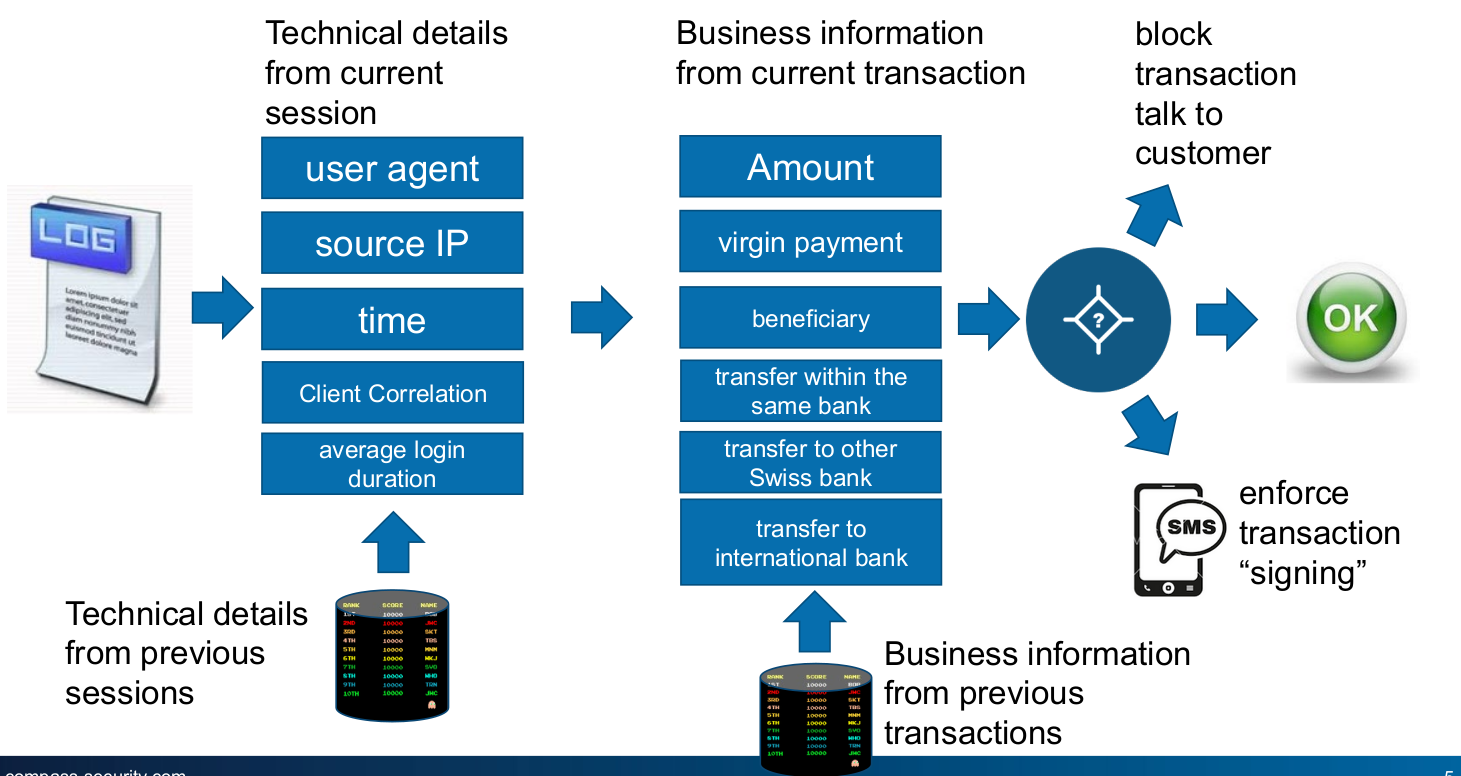
\includegraphics[width=\textwidth]{resources/12-fraud-detection-system.png}
  \caption{Fraud Detection System}
\end{table}

\subsection{E-Mail Security}

\textbf{SPF} (Sender Policy Framework)
\textbf{DKIM} (DomainKeys Identified Mail)
\textbf{DMARC} (Domain-based Message Authentication, Reporting, and Conformance)
DKIM, SPF, and DMARC are all standards that enable different aspects of email authentication. They address complementary issues.
\begin{itemize}
  \item SPF allows senders to define which IP addresses are allowed to send mail for a particular domain.
  \item DKIM provides an encryption key and digital signature that verifies that an email message was not faked or altered.
  \item DMARC unifies the SPF and DKIM authentication mechanisms into a common framework and allows domain owners to declare how they would like email from that domain to be handled if it fails an authorization test.
\end{itemize}

\begin{table}[h]
  \centering
  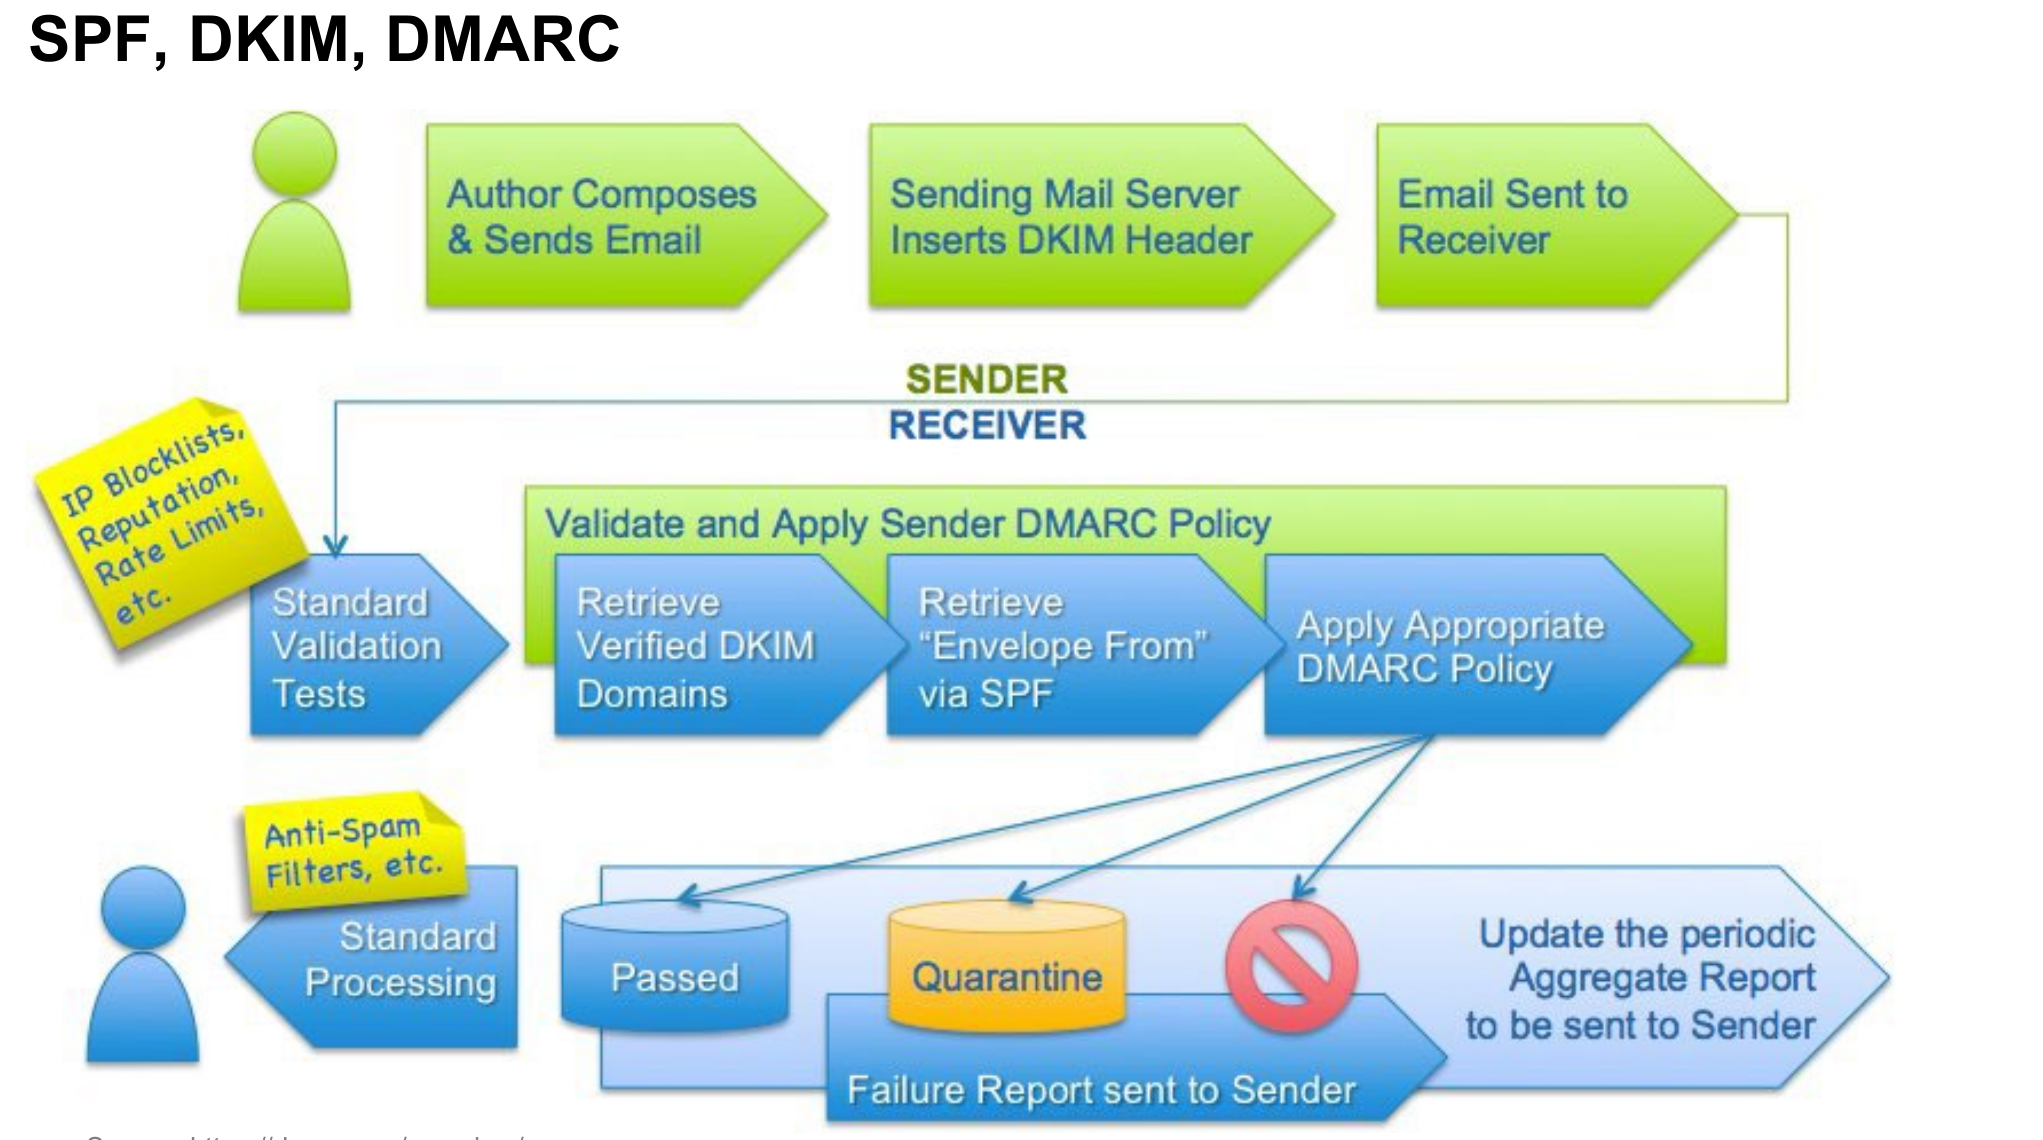
\includegraphics[width=\textwidth]{resources/12-e-mail-security-overview.png}
  \caption{Email Security Overview}
\end{table}

\subsubsection{SPF}
\begin{table}[h]
  \centering
  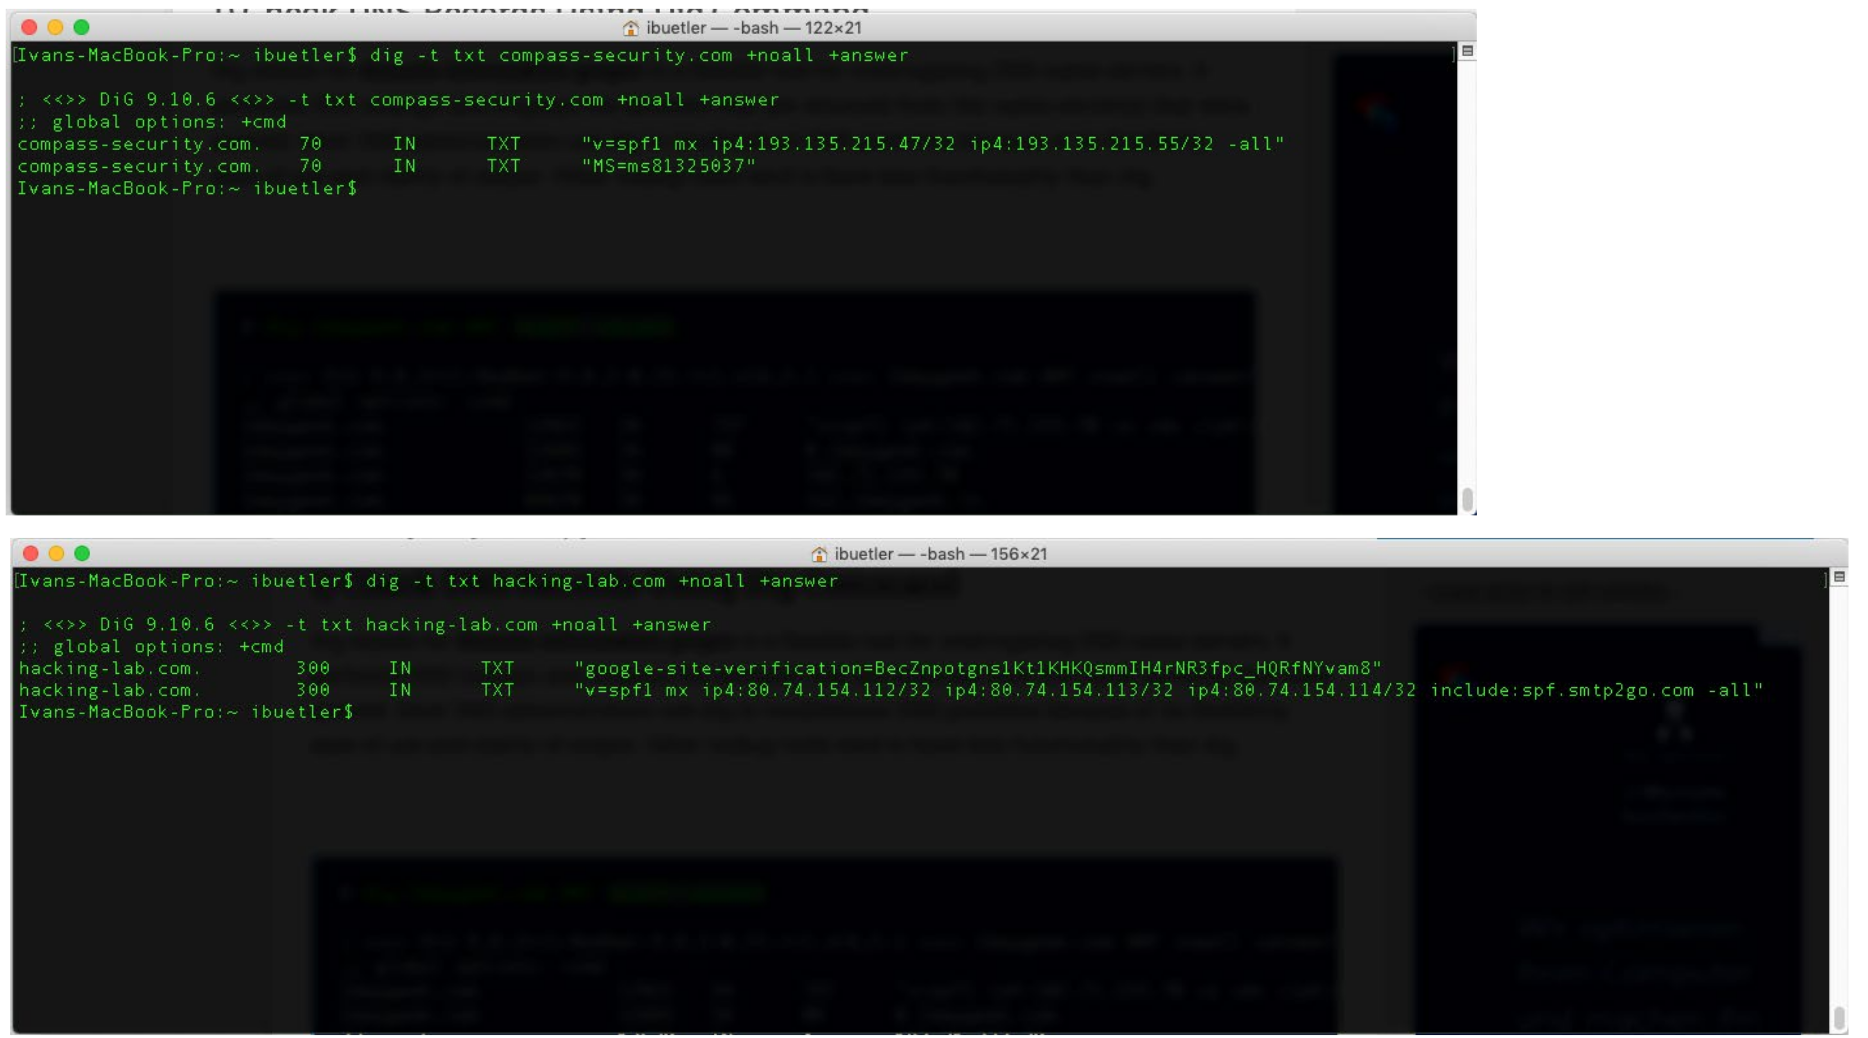
\includegraphics[width=\textwidth]{resources/12-email-security-spf.png}
  \caption{Email Security SPF for Compass Security and Hacking-Lab}
\end{table}

\subsubsection{SPF}
\begin{table}[h]
  \centering
  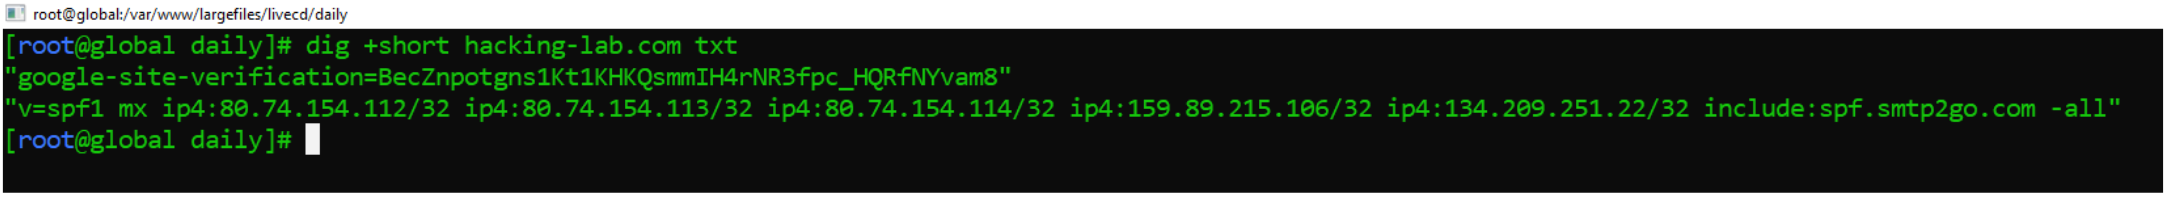
\includegraphics[width=\textwidth]{resources/12-email-security-spf-2.png}
  %\caption{Email Security SPF Query using dig $+$\short}
\end{table}





\subsubsection{DKIM}
DomainKeys Identified Mail, or DKIM, is a technical standard that helps protect email senders and recipients from spam, spoofing, and phishing. It is a form of email authentication that allows an organization to claim responsibility for a message in a way that can be validated by the recipient.

Specifically, it uses an approach called “public key cryptography” to verify that an email message was sent from an authorized mail server, in order to detect forgery and to prevent delivery of harmful email like spam. It supplements SMTP, the basic protocol used to send email, because it does not itself include any authentication mechanisms.


\begin{table}[h]
  \centering
  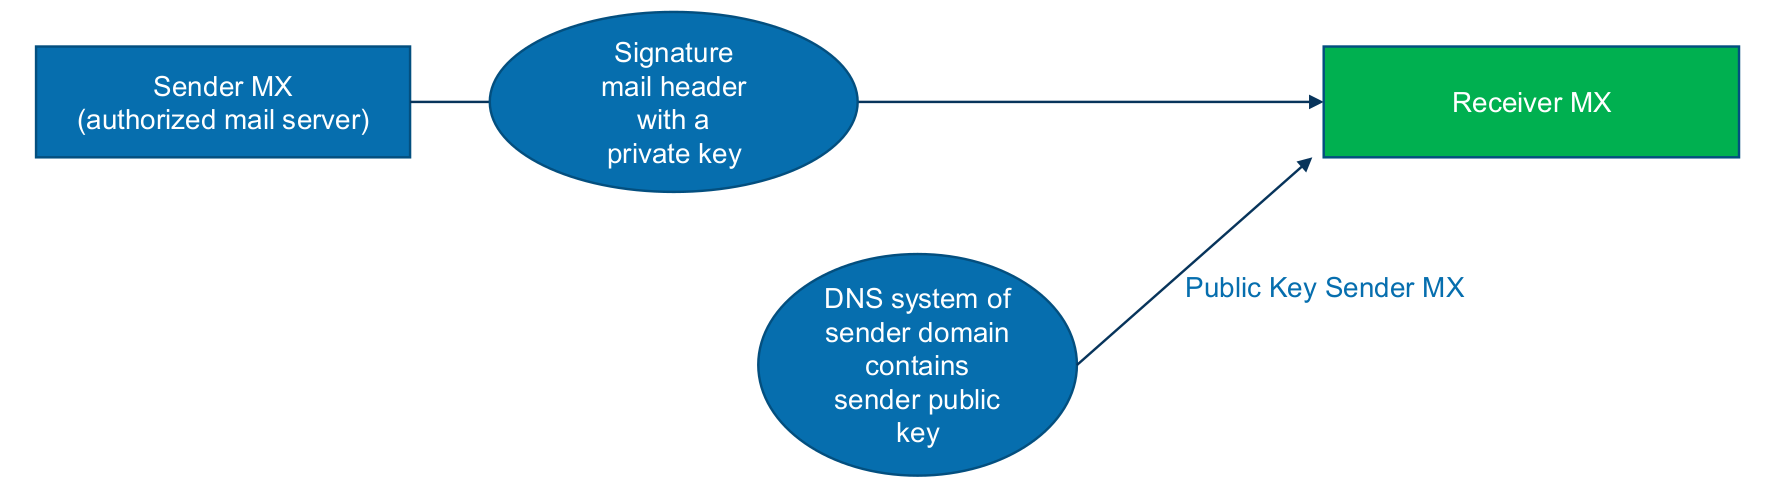
\includegraphics[width=\textwidth]{resources/12-email-security-dkim.png}
  \caption{Email Security DKIM flow}
\end{table}

\begin{table}[h]
  \centering
  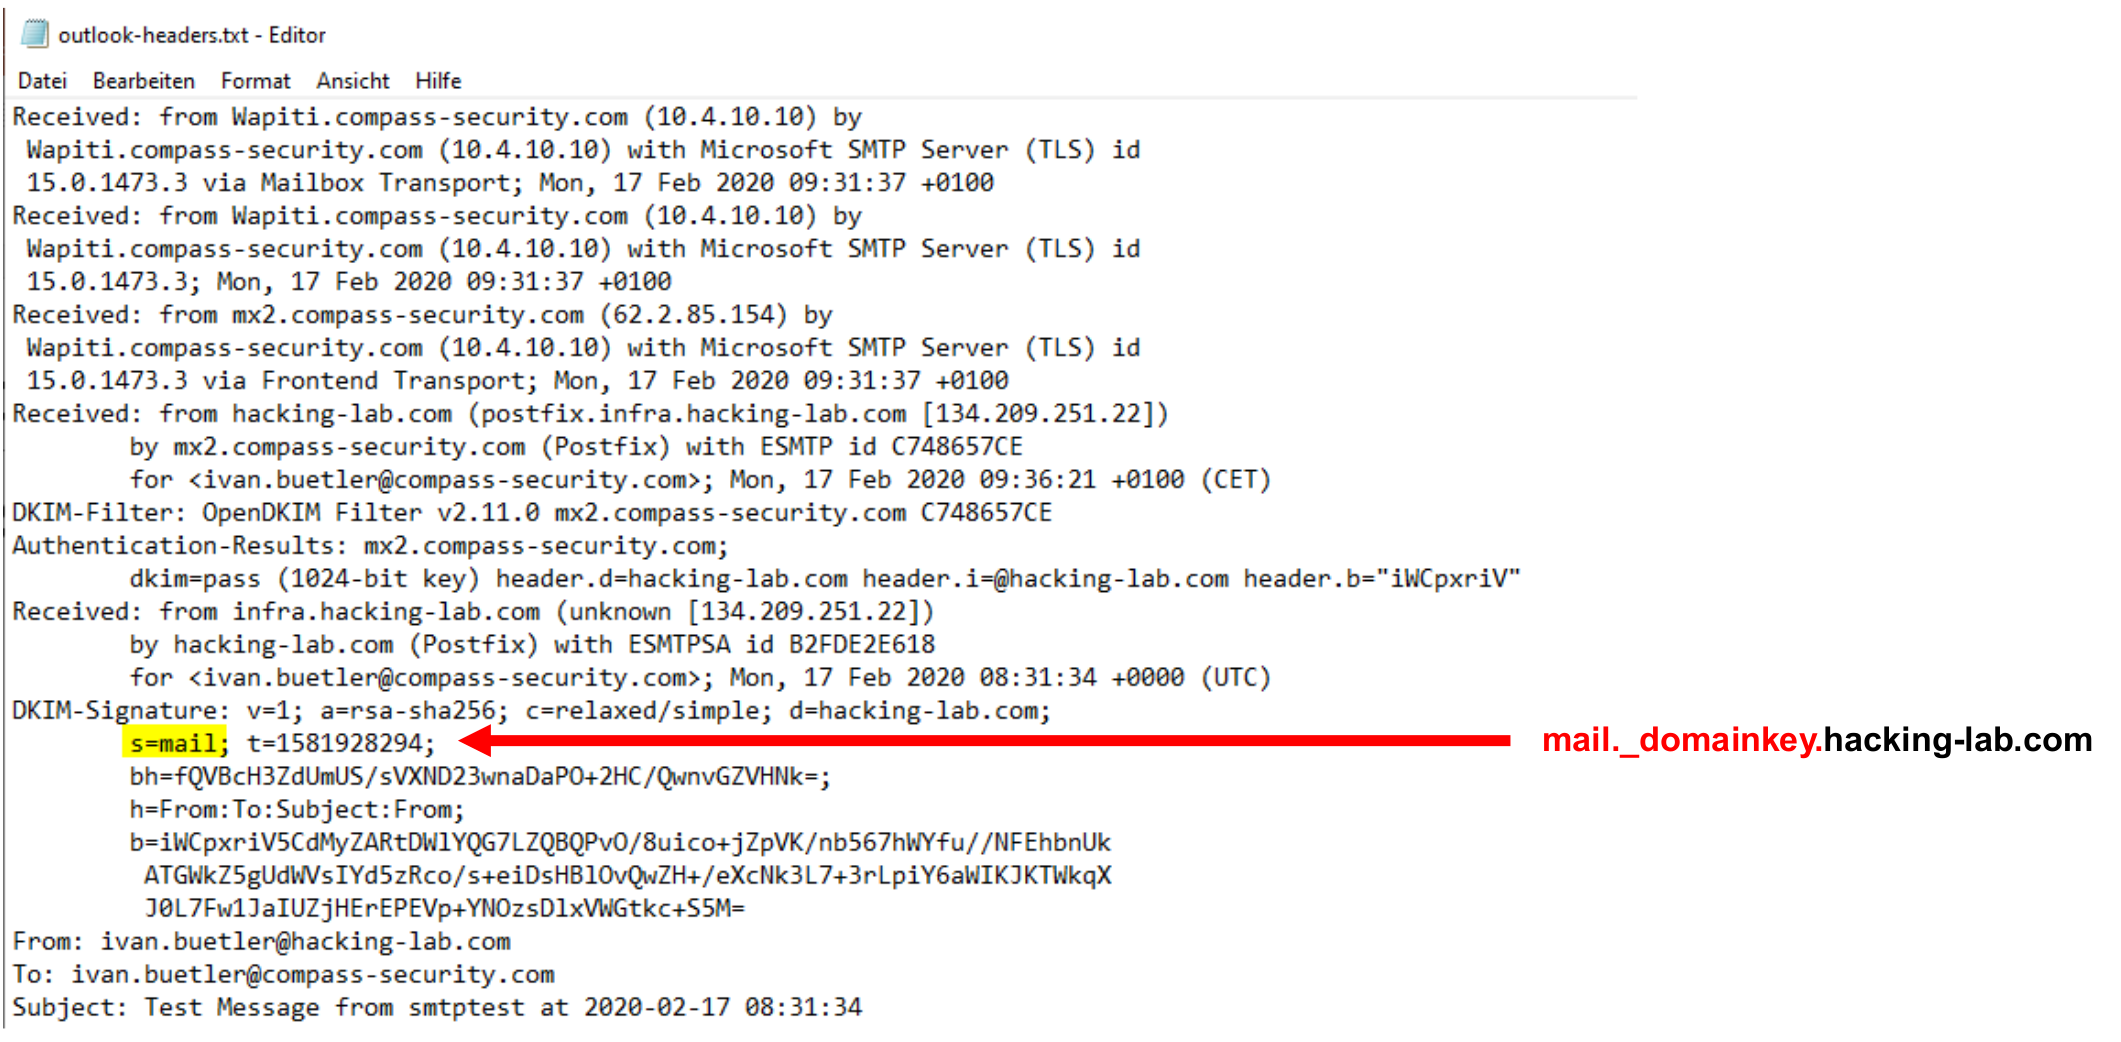
\includegraphics[width=\textwidth]{resources/12-email-security-dkim-2.png}
  \caption{Email Security DKIM mail body example}
\end{table}

\begin{table}[h]
  \centering
  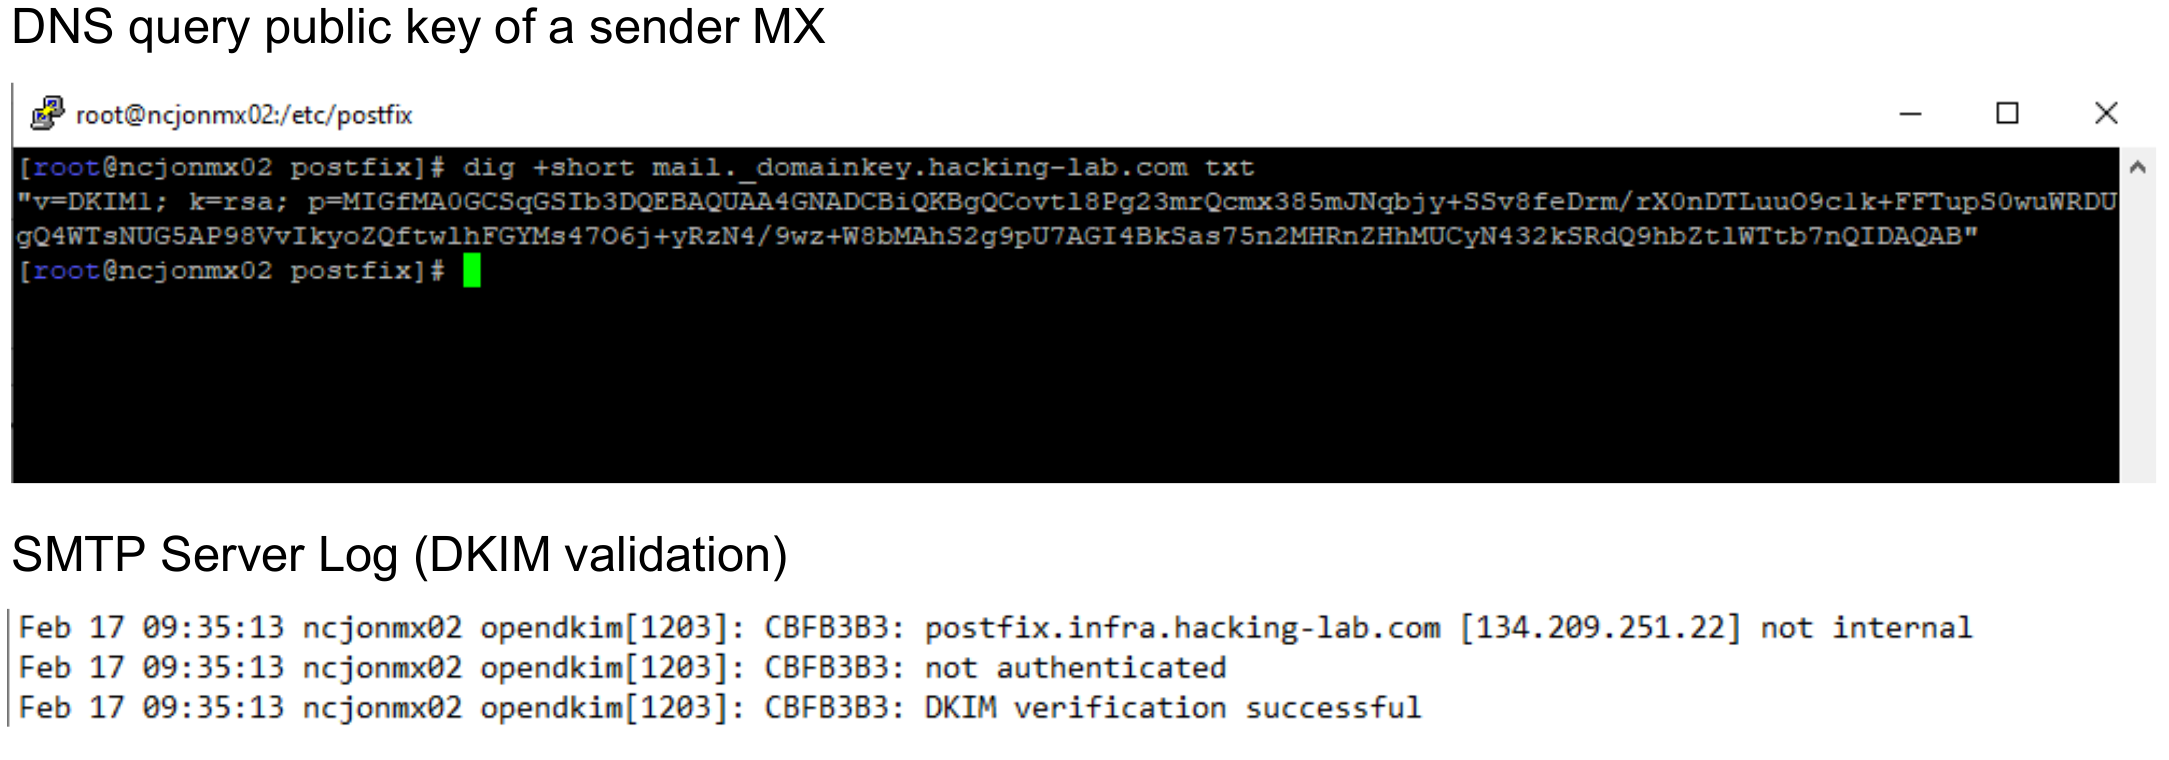
\includegraphics[width=\textwidth]{resources/12-email-security-dkim-3.png}
  \caption{Email Security DKIM dig mx and DKIM validation}
\end{table}

\begin{table}[h]
  \centering
  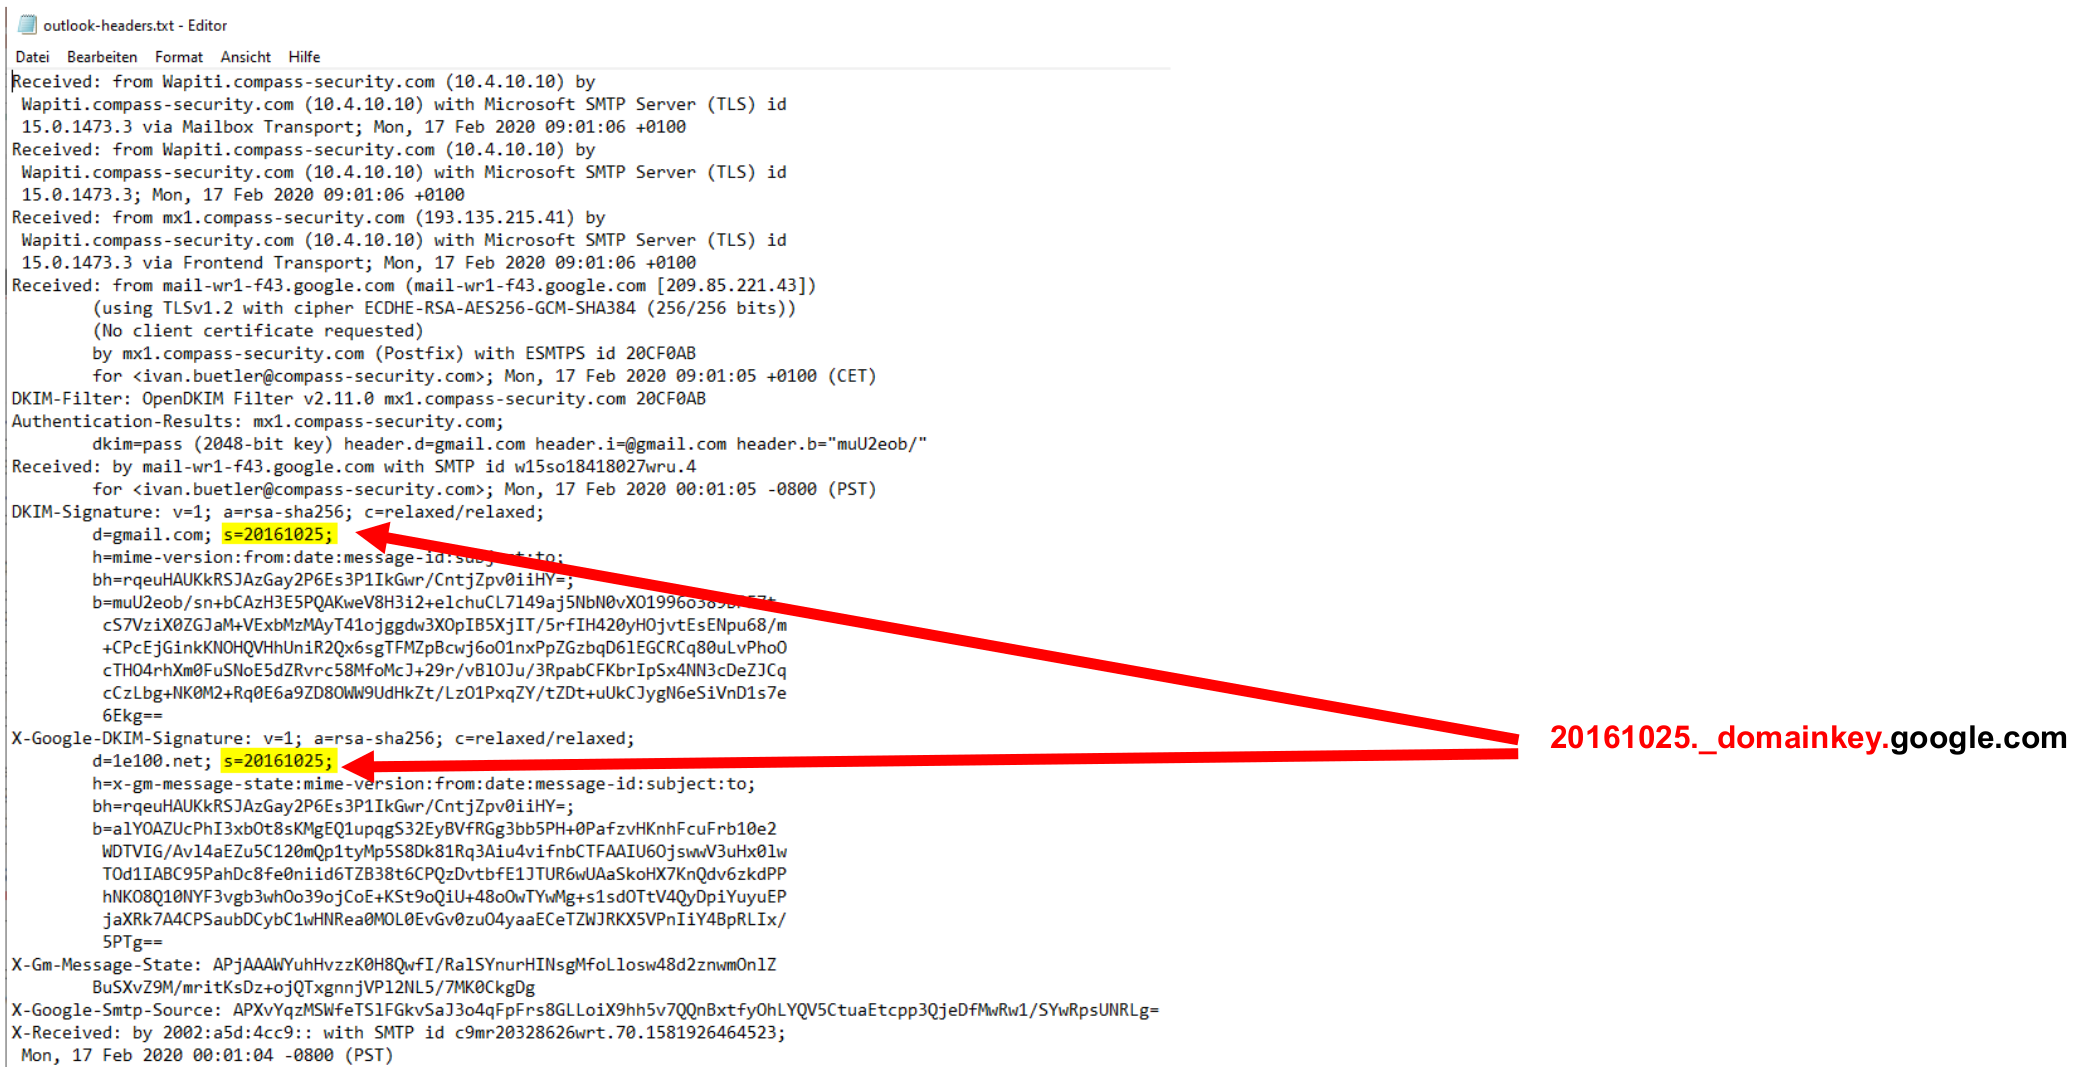
\includegraphics[width=\textwidth]{resources/12-email-security-dkim-4.png}
  \caption{Email Security DKIM GMAIL example}
\end{table}


\begin{table}[h]
  \centering
  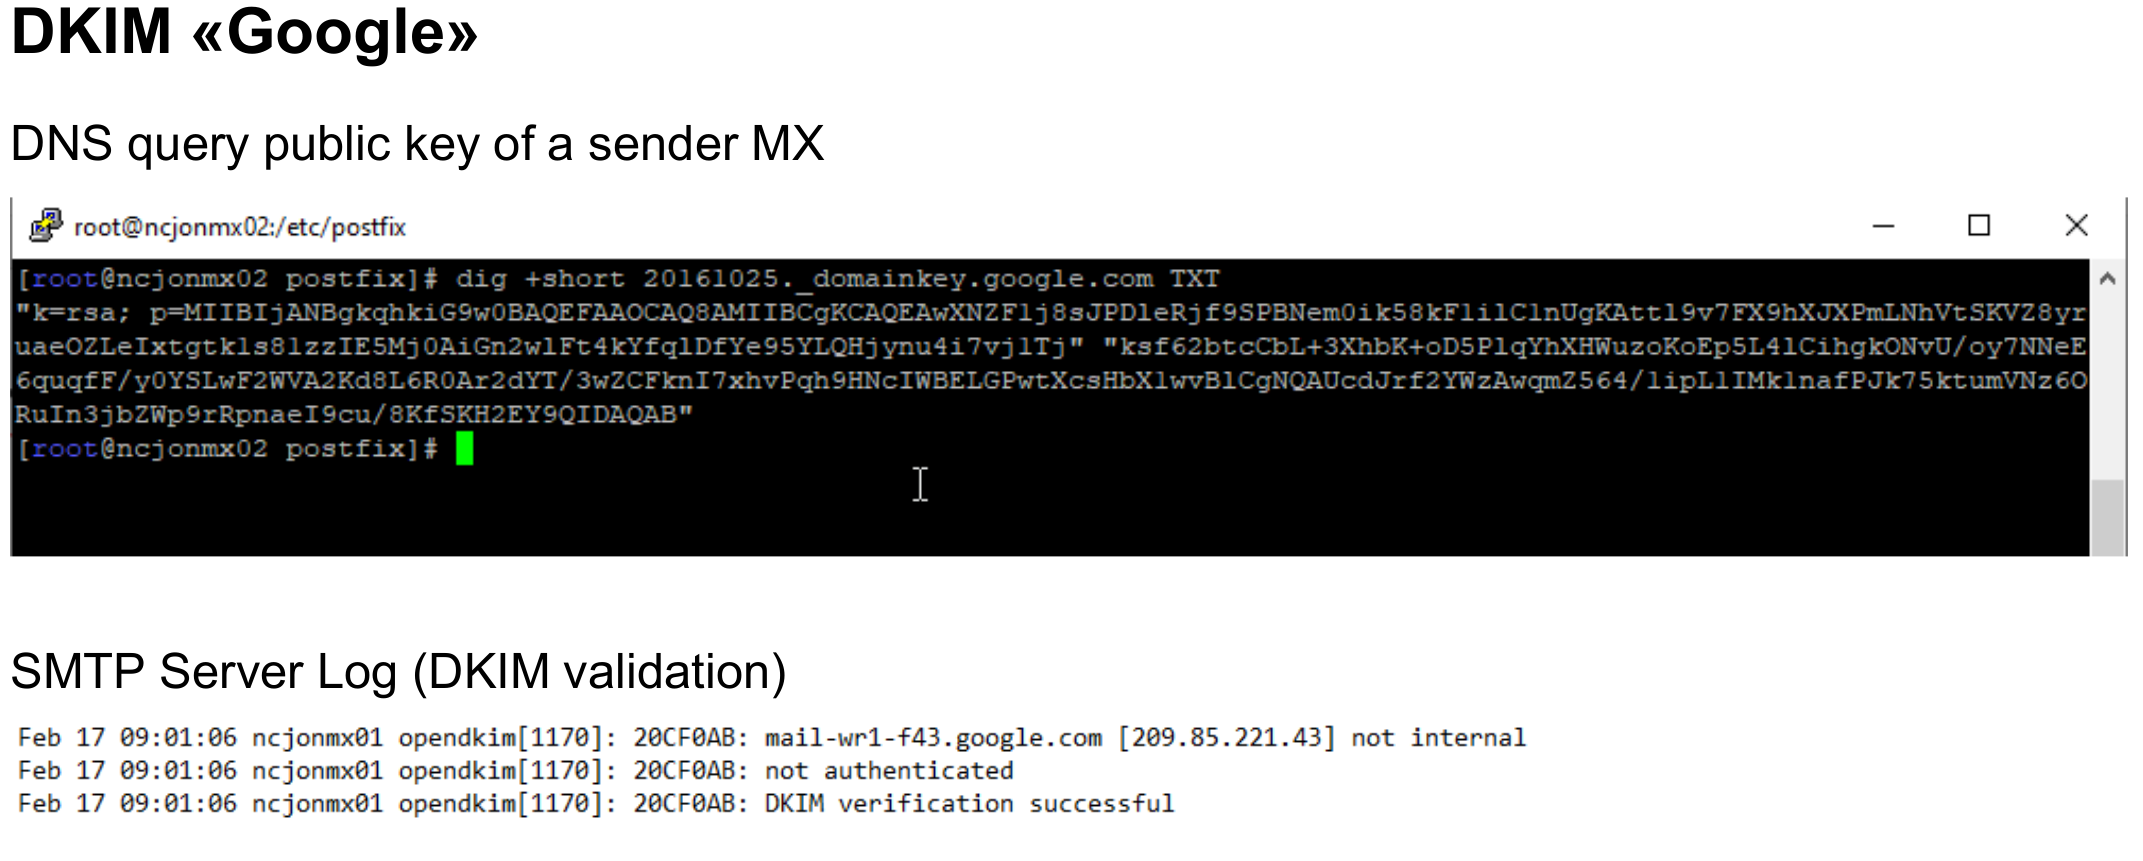
\includegraphics[width=\textwidth]{resources/12-email-security-dkim-5.png}
  \caption{Email Security DKIM dig mx and DKIM validation}
\end{table}


\subsubsection{DMARC}
\textit{DMARC policies are published in the DNS as text (TXT) resource records (RR) and announce what an email receiver should do with non-aligned mail it receives.}
It works by adding a digital signature to the headers of an email message. That signature can be
validated against a public cryptographic key in the organization's Domain Name System (DNS) records. In general terms, the process works like this:

A domain owner publishes a cryptographic public key as a specially-formatted TXT record in the domain's overall DNS records.

When a mail message is sent by an outbound mail server, the server generates and attaches a unique DKIM signature header to the message. This header includes two cryptographic hashes, one of specified headers, and one of the message body (or part of it). The header contains information about how the signature was generated.

When an inbound mail server receives an incoming email, it looks up the sender's public DKIM key in DNS. The inbound server uses this key to decrypt the signature and compare it against a freshly computed version. If the two values match, the message can be proved to authentic and unaltered in transit.


\subsubsection*{DMARC using dig}
DMARC unifies the SPF and DKIM authentication mechanisms into a common framework and allows domain owners to declare how they would like email from that domain to be handled if it fails an authorization test.

\begin{table}[h]
  \centering
  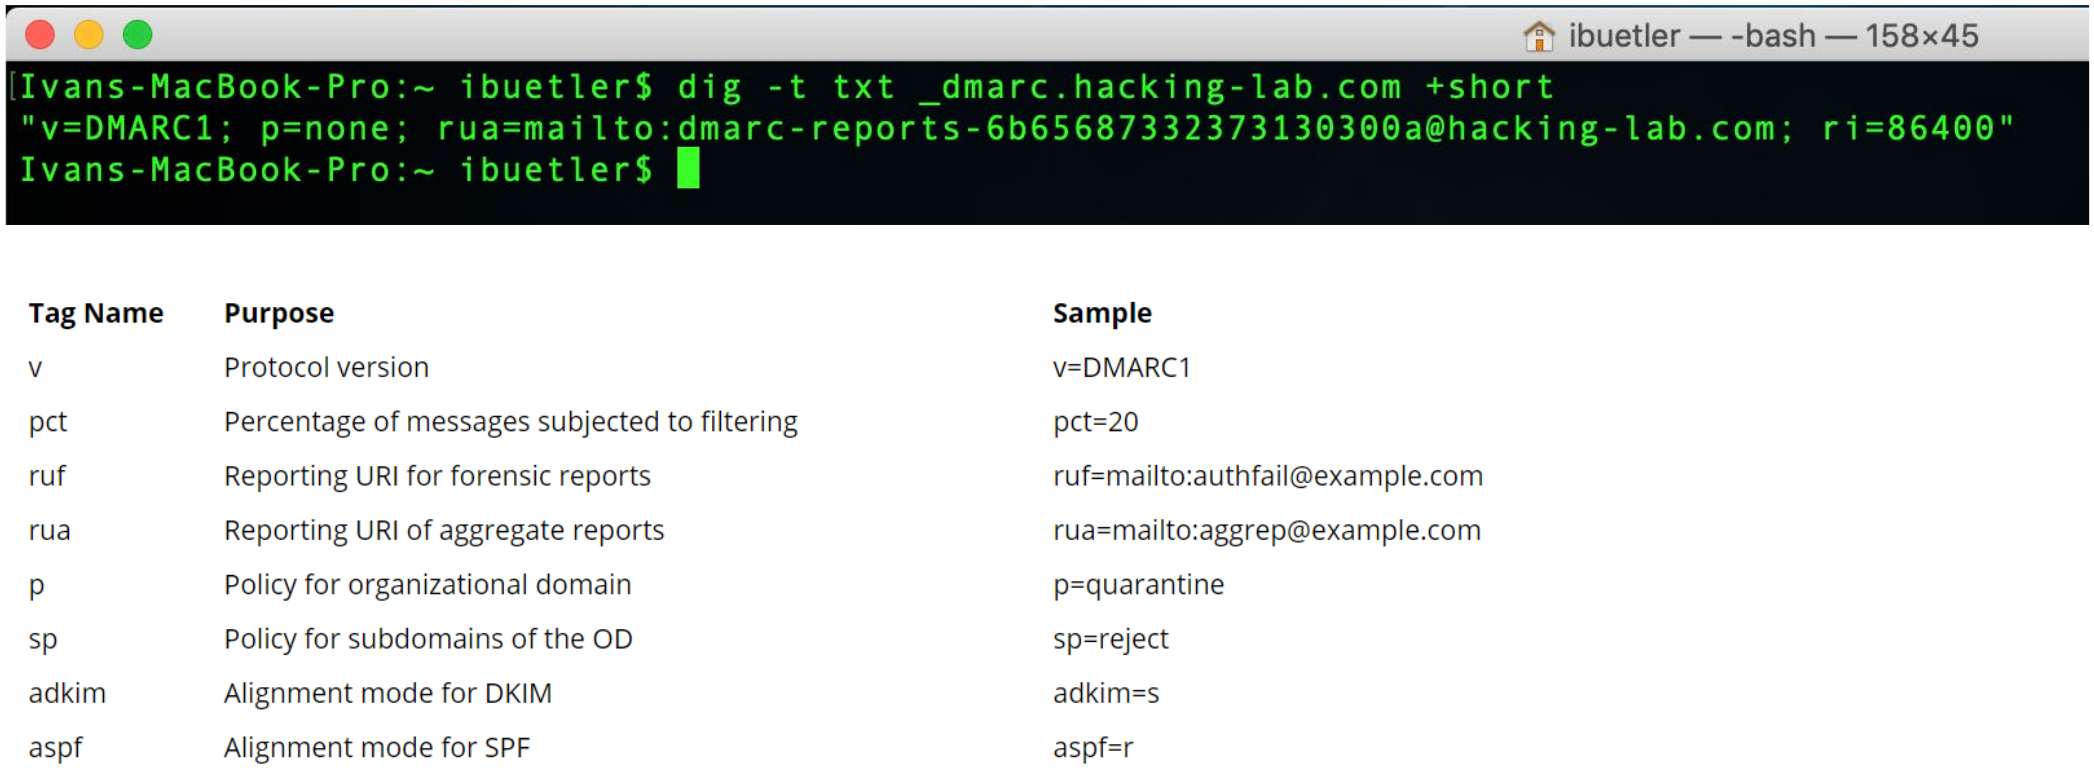
\includegraphics[width=\textwidth]{resources/12-email-security-dmarc.png}
  \caption{Email Security DMARC example dig texting}
\end{table}

\begin{table}[h]
  \centering
  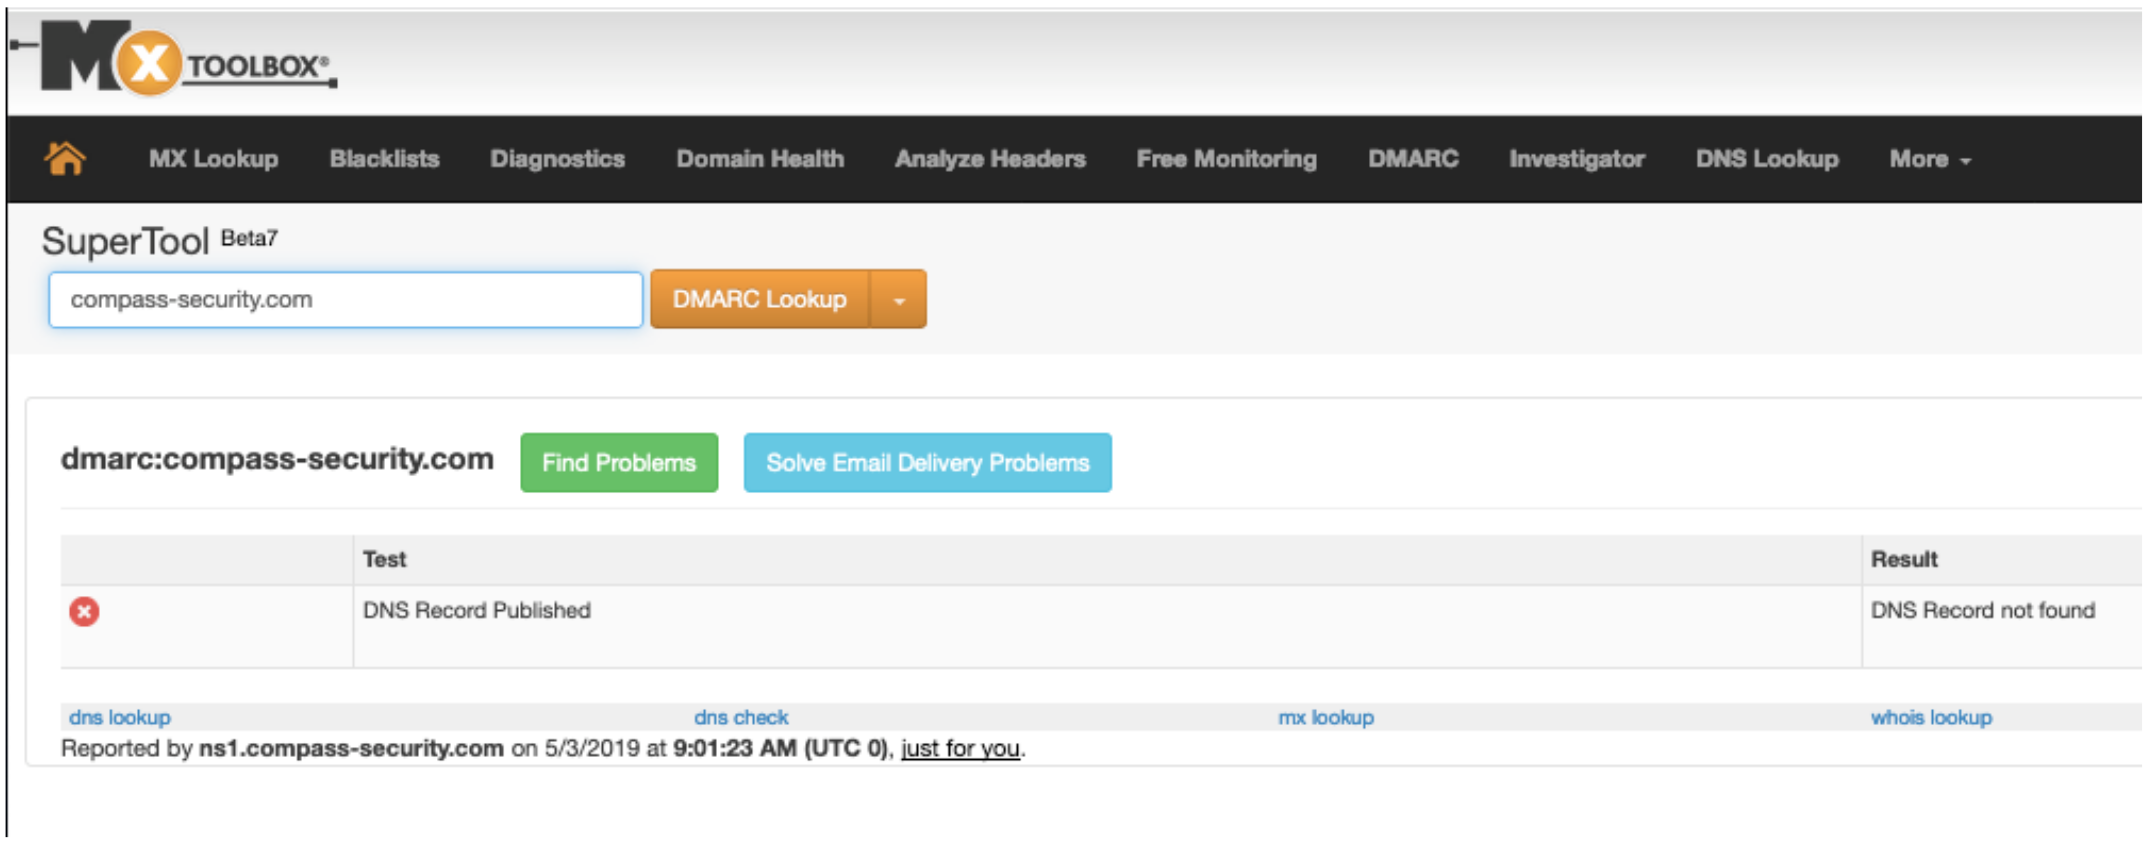
\includegraphics[width=\textwidth]{resources/12-email-security-dmarc-2.png}
  \caption{Email Security DMARC mxtoolbox lookup }
\end{table}

\begin{table}[h]
  \centering
  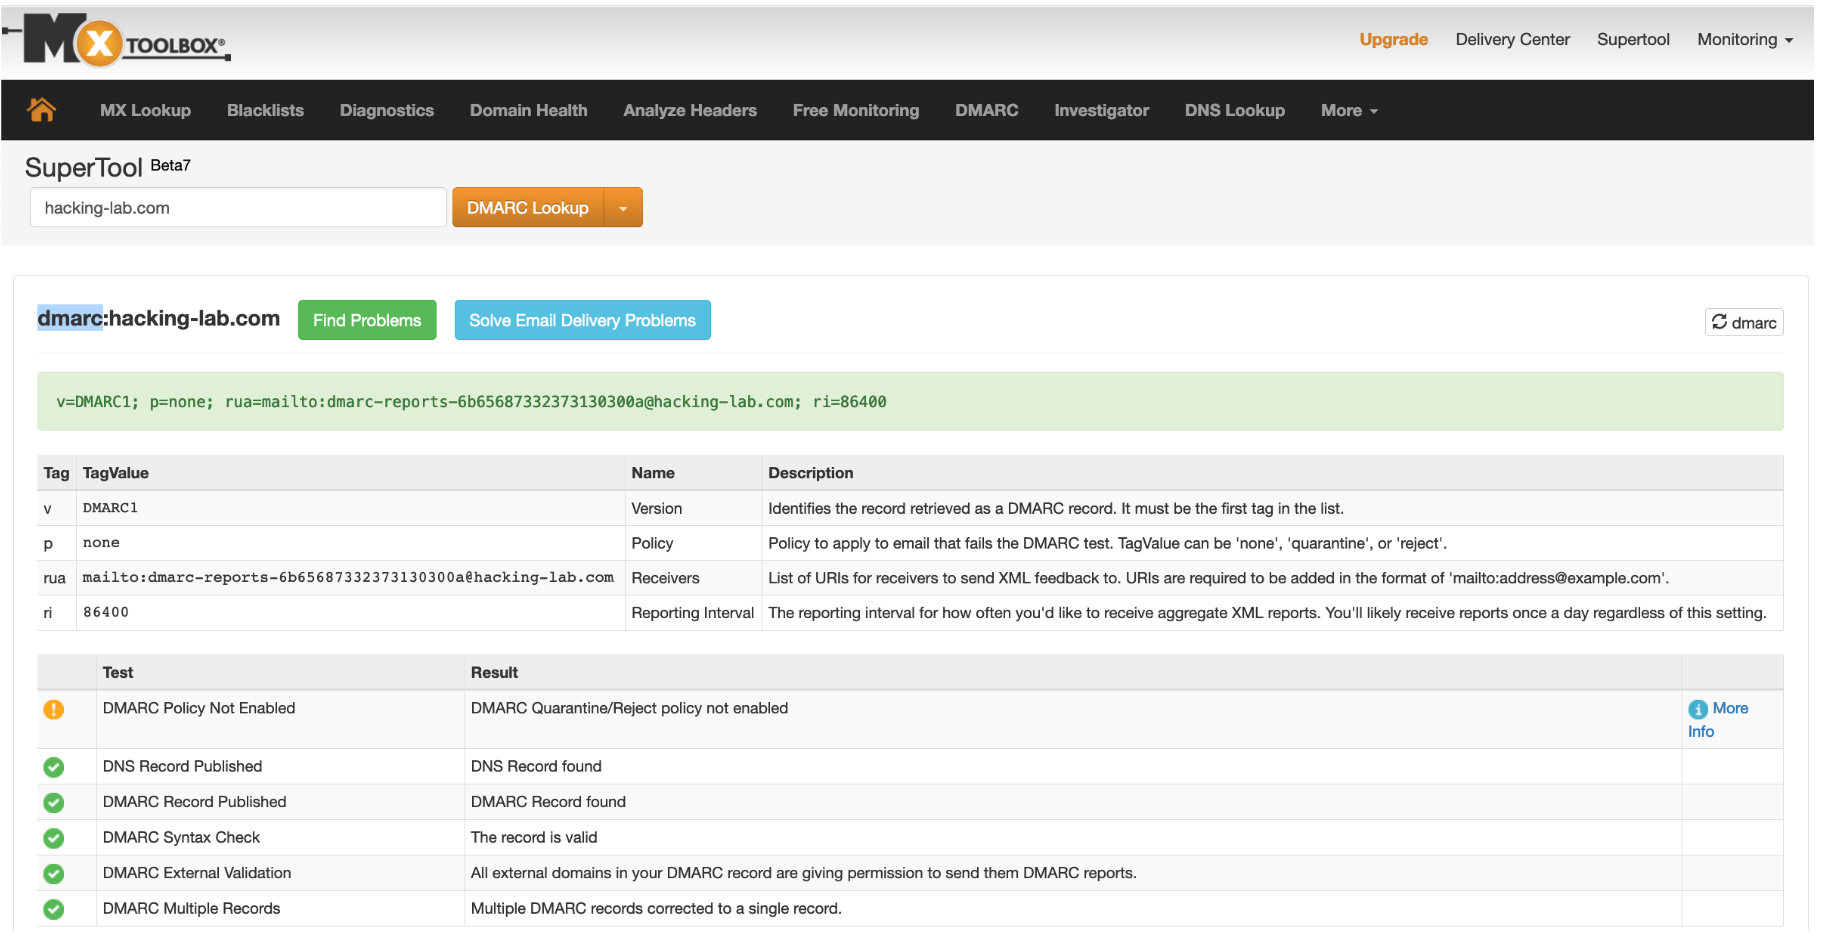
\includegraphics[width=\textwidth]{resources/12-email-security-dmarc-3.png}
  \caption{Email Security DMARC mxtoolbox lookup 2}
\end{table}

\begin{table}[h]
  \centering
  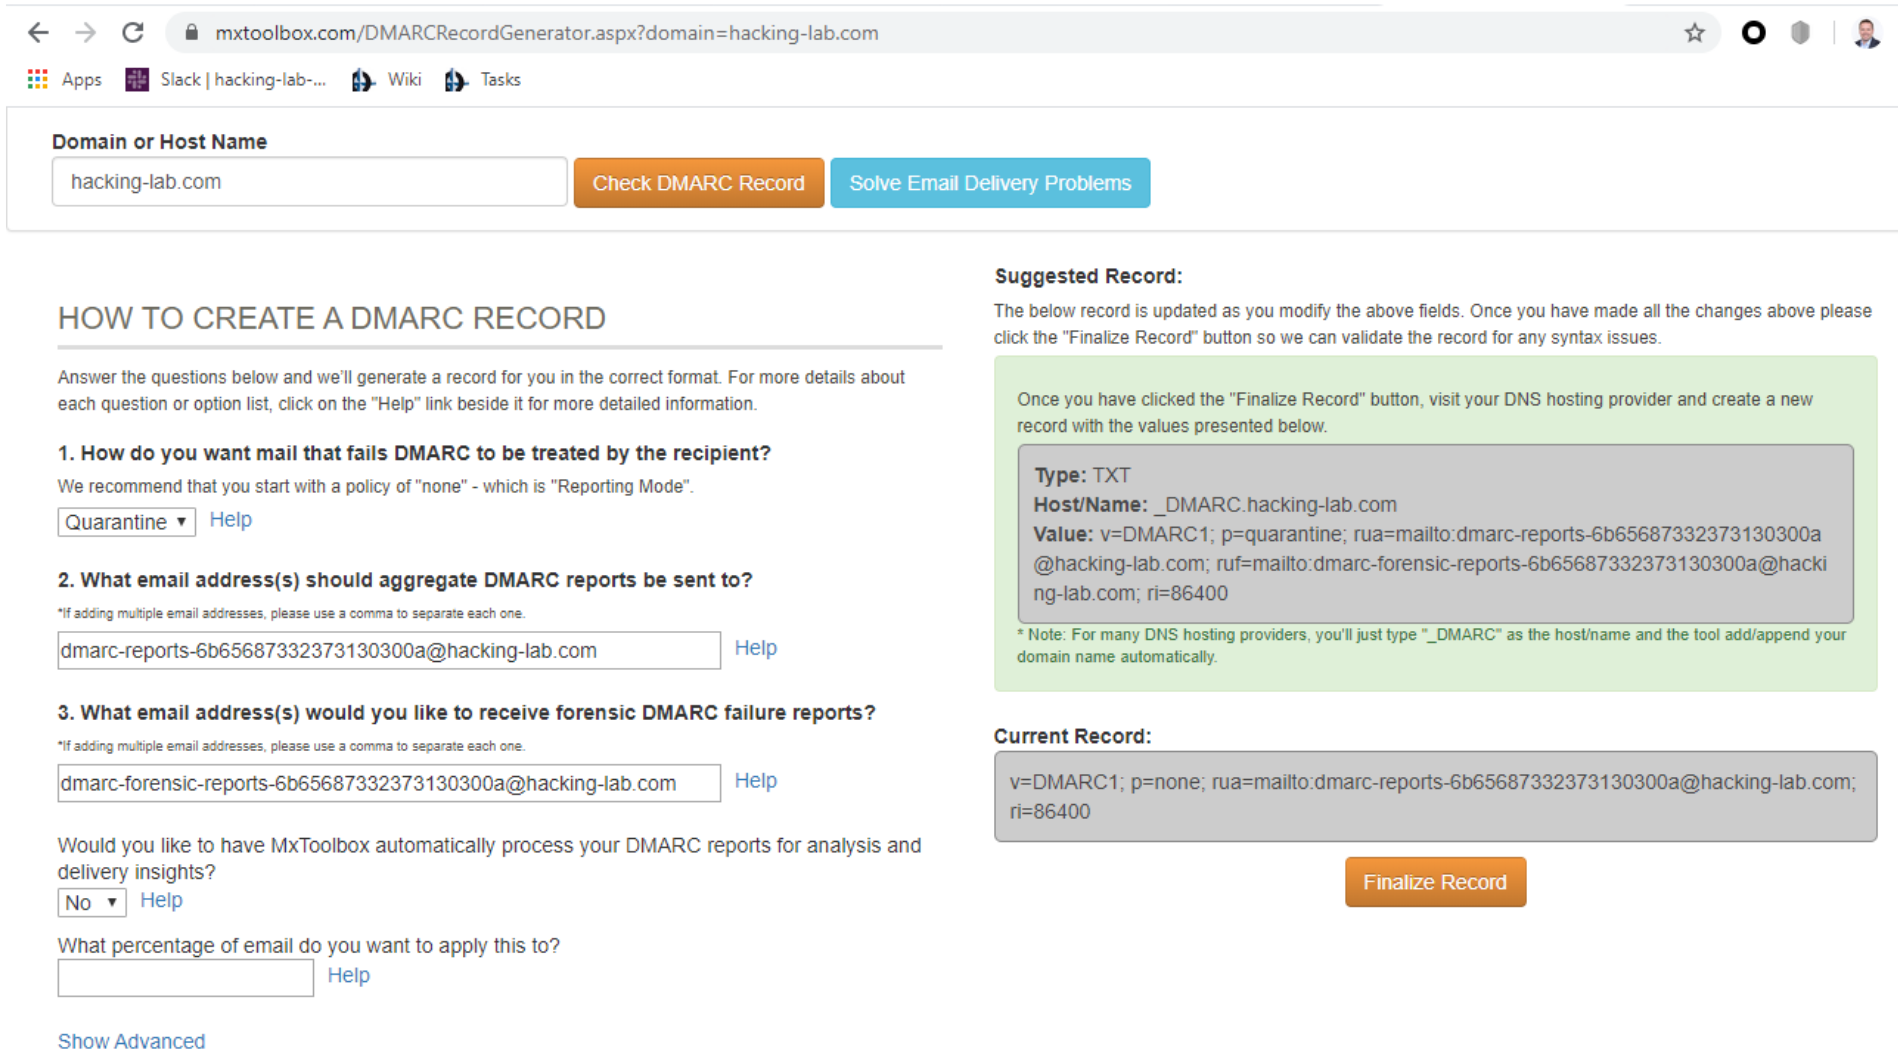
\includegraphics[width=\textwidth]{resources/12-email-security-dmarc-4.png}
  \caption{Email Security DMARC Policy Generator Online} mxtoolbox
\end{table}

\begin{table}[h]
  \centering
  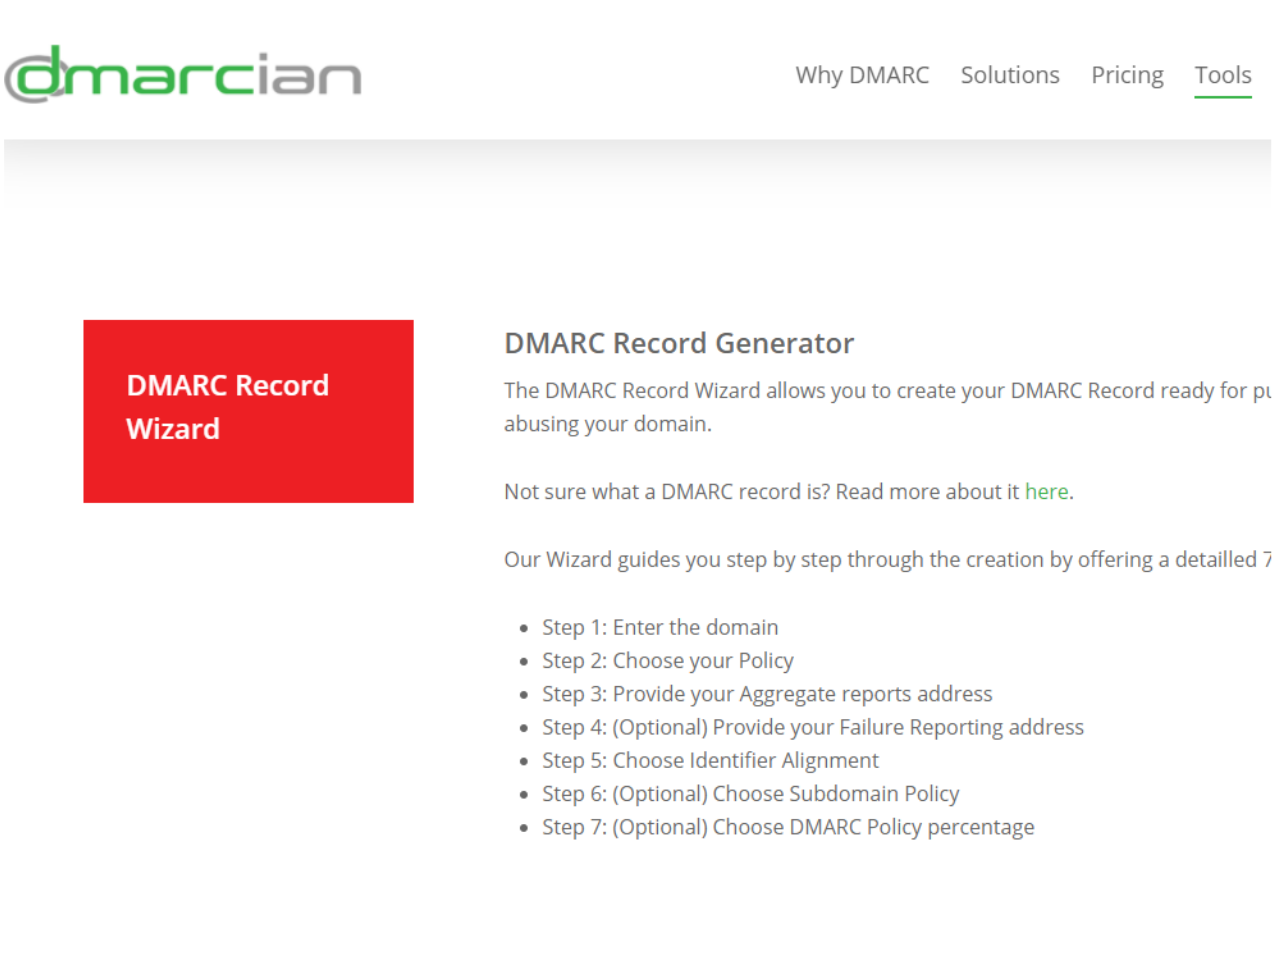
\includegraphics[width=\textwidth]{resources/12-email-security-dmarc-5.png}
  \caption{Email Security DMARC Policy Generator Online dmarcian}
\end{table}

\subsection{Sysmon}
\textit{Windows Monitoring}

\begin{minipage}[t]{0.5\textwidth}
\raggedright
\begin{itemize}
  \item Application log
  \begin{itemize}
    \item Information about applications
  \end{itemize}
  \item System
  \begin{itemize}
    \item System component events
    \item Driver issues, hardware issues...
  \end{itemize}
  \item Security
  \begin{itemize}
    \item Resource use
    \item Logins/logoffs
    \item File access
  \end{itemize}
  \item Also will find a lot under Applications and Services Logs
\end{itemize}\hfill
\end{minipage}
\begin{minipage}[t]{0.45\textwidth}
  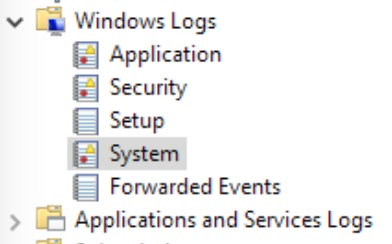
\includegraphics[width=\textwidth]{resources/12-sysmon.png}
\end{minipage}

\subsubsection*{Sexy Six event logs}
\begin{itemize}
  \item 4688/592 (Security) - New Process executed
  \begin{itemize}
    \item Malware or malicious software running, or malicious actor running things
    \item Not every new process is bad!!
    \item Nmap.exe, ssh.exe, psexec.exe, psexecsvc.exe, ping.exe, powershell.exe, etc...
  \end{itemize}
  \item 4624/528/540 (Security) - Account logged in
  \begin{itemize}
    \item Attacker logged in
    \item But not all logins are attackers!
    \item 4625 - Failed logon attempt
  \end{itemize}
  \item 5140/560 (Security) - A share was accessed
  \begin{itemize}
    \item Accessing another computer
    \item Lateral movement
  \end{itemize}

  \item 5156 (Security) - Windows Firewall Network connection by process
  \begin{itemize}
    \item See a process making a connection
    \item Command and control maybe?
  \end{itemize}
  \item 7045/601 (System) - New Service installed
  \begin{itemize}
    \item New services generally should only be installed during patches and new software installation
    \item Change management procedures - helps anomalies stand out
  \end{itemize}
  \item 4663/567 (Security) - File and Registry auditing
  \begin{itemize}
    \item Modifications to the system
    \item Files added
    \item Must enable file auditing
  \end{itemize}

  \item 4720 (Security) – A user account was created
  \begin{itemize}
    \item Attackers could create themselves an account as a backdoor
    \item Should be fairly easy to deconflict with the admin team
  \end{itemize}
  \item 4732/4728 (Security) - A member was added to a group
  \begin{itemize}
    \item Attackers could add their account to a higher privileged account
    \item Should be fairly easy to deconflict with the admin team
  \end{itemize}
\end{itemize}

\subsubsection*{Logon Types}
Most common log event types found in logs.

\begin{itemize}
  \item 2 - Logon via console
  \item 3 - Network logon
  \item 4 - Batch logon
  \item 5 - Windows service logon
  \item 10 - Remote interactive logon (RDP)
\end{itemize}

\subsubsection*{Process Auditing}
So not everything being audited in 4688 is done by default. With gpedit.msc

This shows how to enable detailed process auditing in Windows, as the default logging in Event ID 4688 (process creation) is basic. Using gpedit.msc, you navigate through Windows Group Policy to enable advanced audit policies for process tracking. This captures important details like command-line arguments, parent processes, and user context - critical information for security monitoring.

When combined with Sysmon, this provides comprehensive visibility into system activities, making it valuable for threat detection and incident response. The enhanced logging helps track potential malicious activities and establish audit trails.

The navigation path is:
Computer Configuration -> Windows Settings -> Security Settings -> Advanced Audit Policy Configuration -> System Audit Policies -> Detailed Tracking -> Audit Process Creation

This shows how to enable command-line logging in Windows audit events, which is essential for security monitoring. Through gpedit.msc (Group Policy Editor), you navigate:

Computer Configuration -> Administrative Templates -> System -> Audit Process Creation

Then enable "Include command line in process creation events". This setting ensures Windows logs the full command-line arguments used when processes are launched, providing crucial visibility into how programs are executed - including potential malicious commands. This complements the process auditing we discussed earlier, adding another layer of detail to Windows security logging.

This feature helps detect and investigate suspicious activity like PowerShell commands, malware execution, or living-off-the-land attacks that abuse legitimate system tools.

\subsubsection{Sysmon}
\begin{itemize}
  \item System Monitor (Sysmon) is a Windows system service and device driver that, once installed on a system, remains resident across system reboots to monitor and log system activity to the Windows event log.
  \item Free!
  \item A part of the Sysinternals Suite
  \item Created by Mark Russinovich
  \item Windows service and driver
  \item Monitoring + logging only - no analysis
  \item Up to you + another tool to do that
\end{itemize}

\subsubsection*{Sysmon Event IDs}
\begin{itemize}
  \item 1 - Process creation
  \item 2 - A process changed a file creation time
  \item 3 - Network connection
  \item 4 - Sysmon service state changed (sysmon was started or stopped)
  \item 5 - Process terminated
  \item 6 - Driver loaded
  \item 7 - Image loaded (module is loaded in a process)
  \item 11 - FileCreate
  \item 12 - Registry Event (Create and Delete)
\end{itemize}

\subsubsection*{Installing Sysmon}
\begin{itemize}
  \item Sysmon.exe -accepteula -i
  \item Must install as an admin, since you are installing a service
\end{itemize}

\begin{table}[h]
  \centering
  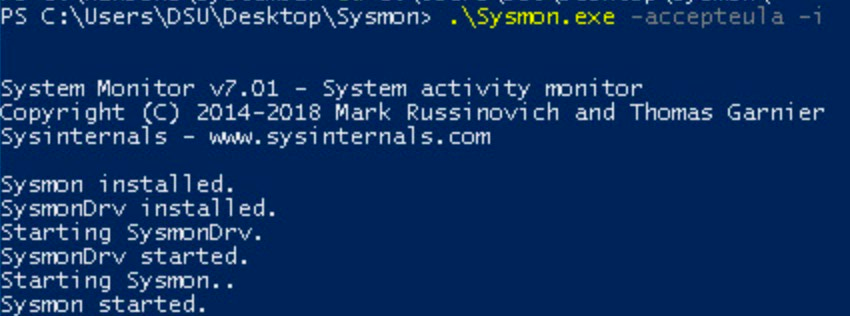
\includegraphics[width=\textwidth]{resources/12-sysmon-installing-sysmon.png}
  \caption{Sysmon installing sysmon}
\end{table}

\begin{itemize}
  \item Sysmon.exe -c
  \item Gets current configuration, not a whole lot.
\end{itemize}
\begin{table}[h]
  \centering
  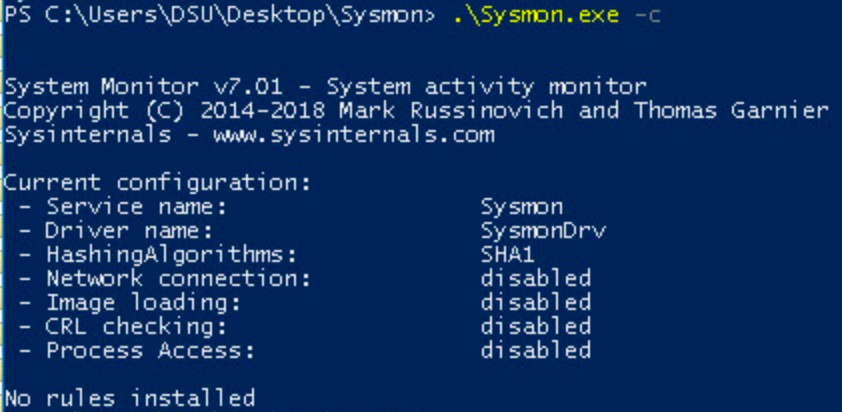
\includegraphics[width=\textwidth]{resources/12-sysmon-default-config.png}
  \caption{Sysmon - default config}
\end{table}

\subsubsection*{Filtering}
\begin{itemize}
  \item We can configure Sysmon to
  \begin{itemize}
    \item Only show certain events (include)
    \item Filter out certain events (exclude)
  \end{itemize}
  \item Do I care to see every smss.exe event?
  \begin{itemize}
    \item Is it malicious?
    \item Probably not... - But make sure you only filter out the OFFICIAL path/executable!
    \item Session Manager Subsystem - it's normal.
  \end{itemize}
  \item XML configuration file
  \begin{itemize}
    \item Include events that match...
    \item Exclude events that match...
  \end{itemize}
\end{itemize}

\subsubsection*{Sample Configuration}

\begin{itemize}
  \item Network
  \begin{itemize}
    \item Only connections on ports 80 and 443 notfrom Internet Explorer
  \end{itemize}
  \item Drivers
  \begin{itemize}
    \item Exclude “Microsoft”
    \item Exclude “windows”
  \end{itemize}
  \item No process termination events
\end{itemize}

\begin{table}[h]
  \centering
  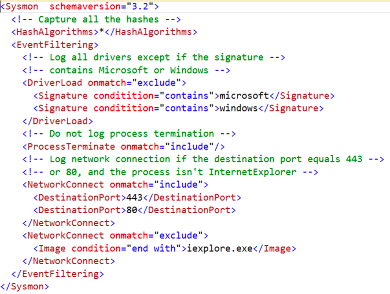
\includegraphics[width=\textwidth]{resources/12-sysmon-sample-config.png}
  \caption{Sysmon - sample config}
\end{table}

\subsubsection*{filtering tempaltes}

\begin{itemize}
  \item SwiftOnSecurity Sysmon Configuration
  \item A good baseline to begin from
  \item 800+ lines
  \begin{itemize}
    \item It's long
    \item But it's good
  \end{itemize}
  \item Tweak for your own organization
\end{itemize}

\subsubsection*{Tweaking the config}
\begin{itemize}
  \item Logging EVERYTHING will get noisy
  \begin{itemize}
    \item Think tons of events on thousands of computers in a large organization
    \item Too much data to deal with
  \end{itemize}
  \item Don't want to exclude things that could be malicious
  \item Please - read through the sample config if you start there
  \begin{itemize}
    \item Make sure you understand what you're doing
    \item Make sure you agree with what it's doing
  \end{itemize}
  \item Put it in play and see what happens
  \begin{itemize}
    \item Some legitimate process making tons of logs on your network? Exclude it.
    \item Afraid you're not getting a full enough picture of something? Include it.
  \end{itemize}
\end{itemize}

\section{exercise}

